\PassOptionsToPackage{unicode=true}{hyperref} % options for packages loaded elsewhere
\PassOptionsToPackage{hyphens}{url}
\documentclass[9pt,ignorenonframetext,aspectratio=169]{beamer}
\IfFileExists{pgfpages.sty}{\usepackage{pgfpages}}{}
\setbeamertemplate{caption}[numbered]
\setbeamertemplate{caption label separator}{: }
\setbeamercolor{caption name}{fg=normal text.fg}
\beamertemplatenavigationsymbolsempty
\usepackage{lmodern}
\usepackage{amssymb,amsmath}
\usepackage{ifxetex,ifluatex}
\usepackage{fixltx2e} % provides \textsubscript
\ifnum 0\ifxetex 1\fi\ifluatex 1\fi=0 % if pdftex
  \usepackage[T1]{fontenc}
  \usepackage[utf8]{inputenc}
\else % if luatex or xelatex
  \ifxetex
    \usepackage{mathspec}
  \else
    \usepackage{fontspec}
\fi
\defaultfontfeatures{Ligatures=TeX,Scale=MatchLowercase}







\fi

  \usetheme[]{metropolis}






% use upquote if available, for straight quotes in verbatim environments
\IfFileExists{upquote.sty}{\usepackage{upquote}}{}
% use microtype if available
\IfFileExists{microtype.sty}{%
  \usepackage{microtype}
  \UseMicrotypeSet[protrusion]{basicmath} % disable protrusion for tt fonts
}{}


\newif\ifbibliography
  \usepackage[style=abnt,]{biblatex}
      \addbibresource{references.bib}
  

\hypersetup{
      pdftitle={Crítica ao uso do Campo de Arbítrio do Avaliador},
        pdfauthor={Luiz Fernando Palin Droubi ; Carlos Augusto Zilli ; Willian Zonato ; Norberto Hochheim},
          pdfborder={0 0 0},
    breaklinks=true}
%\urlstyle{same}  % Use monospace font for urls







% Prevent slide breaks in the middle of a paragraph:
\widowpenalties 1 10000
\raggedbottom

  \AtBeginPart{
    \let\insertpartnumber\relax
    \let\partname\relax
    \frame{\partpage}
  }
  \AtBeginSection{
    \ifbibliography
    \else
      \let\insertsectionnumber\relax
      \let\sectionname\relax
      \frame{\sectionpage}
    \fi
  }
  \AtBeginSubsection{
    \let\insertsubsectionnumber\relax
    \let\subsectionname\relax
    \frame{\subsectionpage}
  }



\setlength{\parindent}{0pt}
\setlength{\parskip}{6pt plus 2pt minus 1pt}
\setlength{\emergencystretch}{3em}  % prevent overfull lines
\providecommand{\tightlist}{%
  \setlength{\itemsep}{0pt}\setlength{\parskip}{0pt}}

  \setcounter{secnumdepth}{0}


  \usepackage[brazil]{babel}
  \usepackage{csquotes}

  \title[]{Crítica ao uso do Campo de Arbítrio do Avaliador}

  \subtitle{em situações de escassez de dados de mercado}

  \author[
        Luiz Fernando Palin Droubi\footnote<.->{\href{mailto:lfpdroubi@gmail.com}{\nolinkurl{lfpdroubi@gmail.com}}}
\newline \and Carlos Augusto Zilli\footnote<.->{\href{mailto:carlos.zilli@ifsc.edu.br}{\nolinkurl{carlos.zilli@ifsc.edu.br}}}
\newline \and Willian Zonato\footnote<.->{\href{mailto:will.zonato@gmail.com}{\nolinkurl{will.zonato@gmail.com}}}
\newline \and Norberto Hochheim\footnote<.->{\href{mailto:norberto.hochheim@ufsc.br}{\nolinkurl{norberto.hochheim@ufsc.br}}}
    ]{Luiz Fernando Palin Droubi\footnote<.->{\href{mailto:lfpdroubi@gmail.com}{\nolinkurl{lfpdroubi@gmail.com}}}
\newline \and Carlos Augusto Zilli\footnote<.->{\href{mailto:carlos.zilli@ifsc.edu.br}{\nolinkurl{carlos.zilli@ifsc.edu.br}}}
\newline \and Willian Zonato\footnote<.->{\href{mailto:will.zonato@gmail.com}{\nolinkurl{will.zonato@gmail.com}}}
\newline \and Norberto Hochheim\footnote<.->{\href{mailto:norberto.hochheim@ufsc.br}{\nolinkurl{norberto.hochheim@ufsc.br}}}}

  \institute[
    ]{
    GEAP - UFSC
    }

\date[
      \today
  ]{
      \today
        }


\begin{document}

% Hide progress bar and footline on titlepage
  \begin{frame}[plain]
  \titlepage
  \end{frame}


  \begin{frame}
  \tableofcontents[hideallsubsections]
  \end{frame}

\hypertarget{regressuxe3o-linear}{%
\section{Regressão Linear}\label{regressuxe3o-linear}}

\begin{frame}{Definição}
\protect\hypertarget{definiuxe7uxe3o}{}

\begin{itemize}[<+->]
\tightlist
\item
  A regressão linear é uma função que \emph{estima} o valor da
  \emph{média condicional} de uma população
  \autocite[10-11]{matloff2017}.

  \begin{itemize}[<+->]
  \tightlist
  \item
    P. ex.:

    \begin{itemize}[<+->]
    \tightlist
    \item
      \(VU = \beta_0 + \beta_1A + \beta_2F + \varepsilon\)
    \item
      \(\mu(VU) = \mathbb E [VU|A, F] = \beta_0 + \beta_1A + \beta_2F + \mathbb E[\varepsilon]\)
    \item
      Se \(\varepsilon \approx N(0, \sigma^2)\)
    \item
      \(\mu(VU) = \mathbb E [VU|A, F] = \beta_0 + \beta_1A + \beta_2F\)
    \end{itemize}
  \item
    São estimados
    \(\hat \beta_0, \hat \beta_1, \hat \beta_2 \,e\,\hat \varepsilon\)
  \item
    Caso o modelo seja bem especificado,
    \(\hat \varepsilon^2 \approx \sigma^2\)
  \end{itemize}
\item
  A equação estimada pode ser utilizada para fazer estimativas e
  previsões

  \begin{itemize}[<+->]
  \tightlist
  \item
    P. ex.: Qual o \emph{valor unitário médio} (ou esperado) de um lote,
    dado que ele possui \(A = 360m^2\) e \(F = 12m\)?

    \begin{itemize}[<+->]
    \tightlist
    \item
      \(\mathbb E [VU|A = 360, F = 12] = \hat \beta_0 + \hat \beta_1 \cdot 360 + \hat \beta_2 \cdot 12 + \mathbb E[\hat \varepsilon]\)
    \item
      \(\mathbb E [VU|A = 360, F = 12] = \hat \beta_0 + \hat \beta_1 \cdot 360 + \hat \beta_2 \cdot 12\)
    \item
      Incerteza do estimador deve ser verificada com IC
    \end{itemize}
  \item
    Mas qual o valor de um novo lote, dado que ele possui \(A = 360m^2\)
    e \(F = 12m\)?

    \begin{itemize}[<+->]
    \tightlist
    \item
      \(\hat{VU} = \hat \beta_0 + \hat \beta_1 \cdot 360 + \hat \beta_2 \cdot 12 + \hat \varepsilon\)
    \item
      Incerteza na predição deve ser verificada com IP
    \end{itemize}
  \end{itemize}
\end{itemize}

\end{frame}

\begin{frame}{Função média condicional}
\protect\hypertarget{funuxe7uxe3o-muxe9dia-condicional}{}

\begin{figure}

{\centering 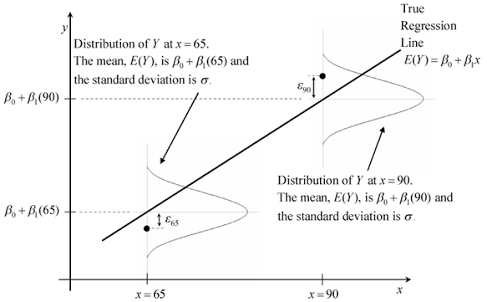
\includegraphics[width=0.7\linewidth]{../../images/RlmM2} 

}

\caption{Médias Condicionais.}\label{fig:unnamed-chunk-1}
\end{figure}

\end{frame}

\begin{frame}{Estimação vs.~previsão de valores}
\protect\hypertarget{estimauxe7uxe3o-vs.-previsuxe3o-de-valores}{}

\begin{itemize}[<+->]
\tightlist
\item
  Sir Francis \textcite[p.~62]{galton}
  \autocite[\emph{apud}][p.~350]{koenker2000} criticou os seus colegas
  que:

  \begin{itemize}[<+->]
  \tightlist
  \item
    \emph{limitam suas investigações a médias, e não parecem se deleitar com
    visões mais abrangentes. Suas almas parecem tão enfadonhas ao encanto da
    variedade quanto ao de um nativo de um de nossos condados ingleses planos, cuja
    retrospectiva da Suíça foi que, se as montanhas pudessem ser jogadas em seus
    lagos, dois incômodos seriam removidos de uma só vez.}
  \end{itemize}
\item
  Estimação é para parâmetros da população (média, variância,
  coeficientes, \ldots)
\item
  Previsão é para novos dados da população (fora da amostra).
\end{itemize}

\end{frame}

\begin{frame}{Estimação: outros quantis de dados}
\protect\hypertarget{estimauxe7uxe3o-outros-quantis-de-dados}{}

\begin{figure}

{\centering 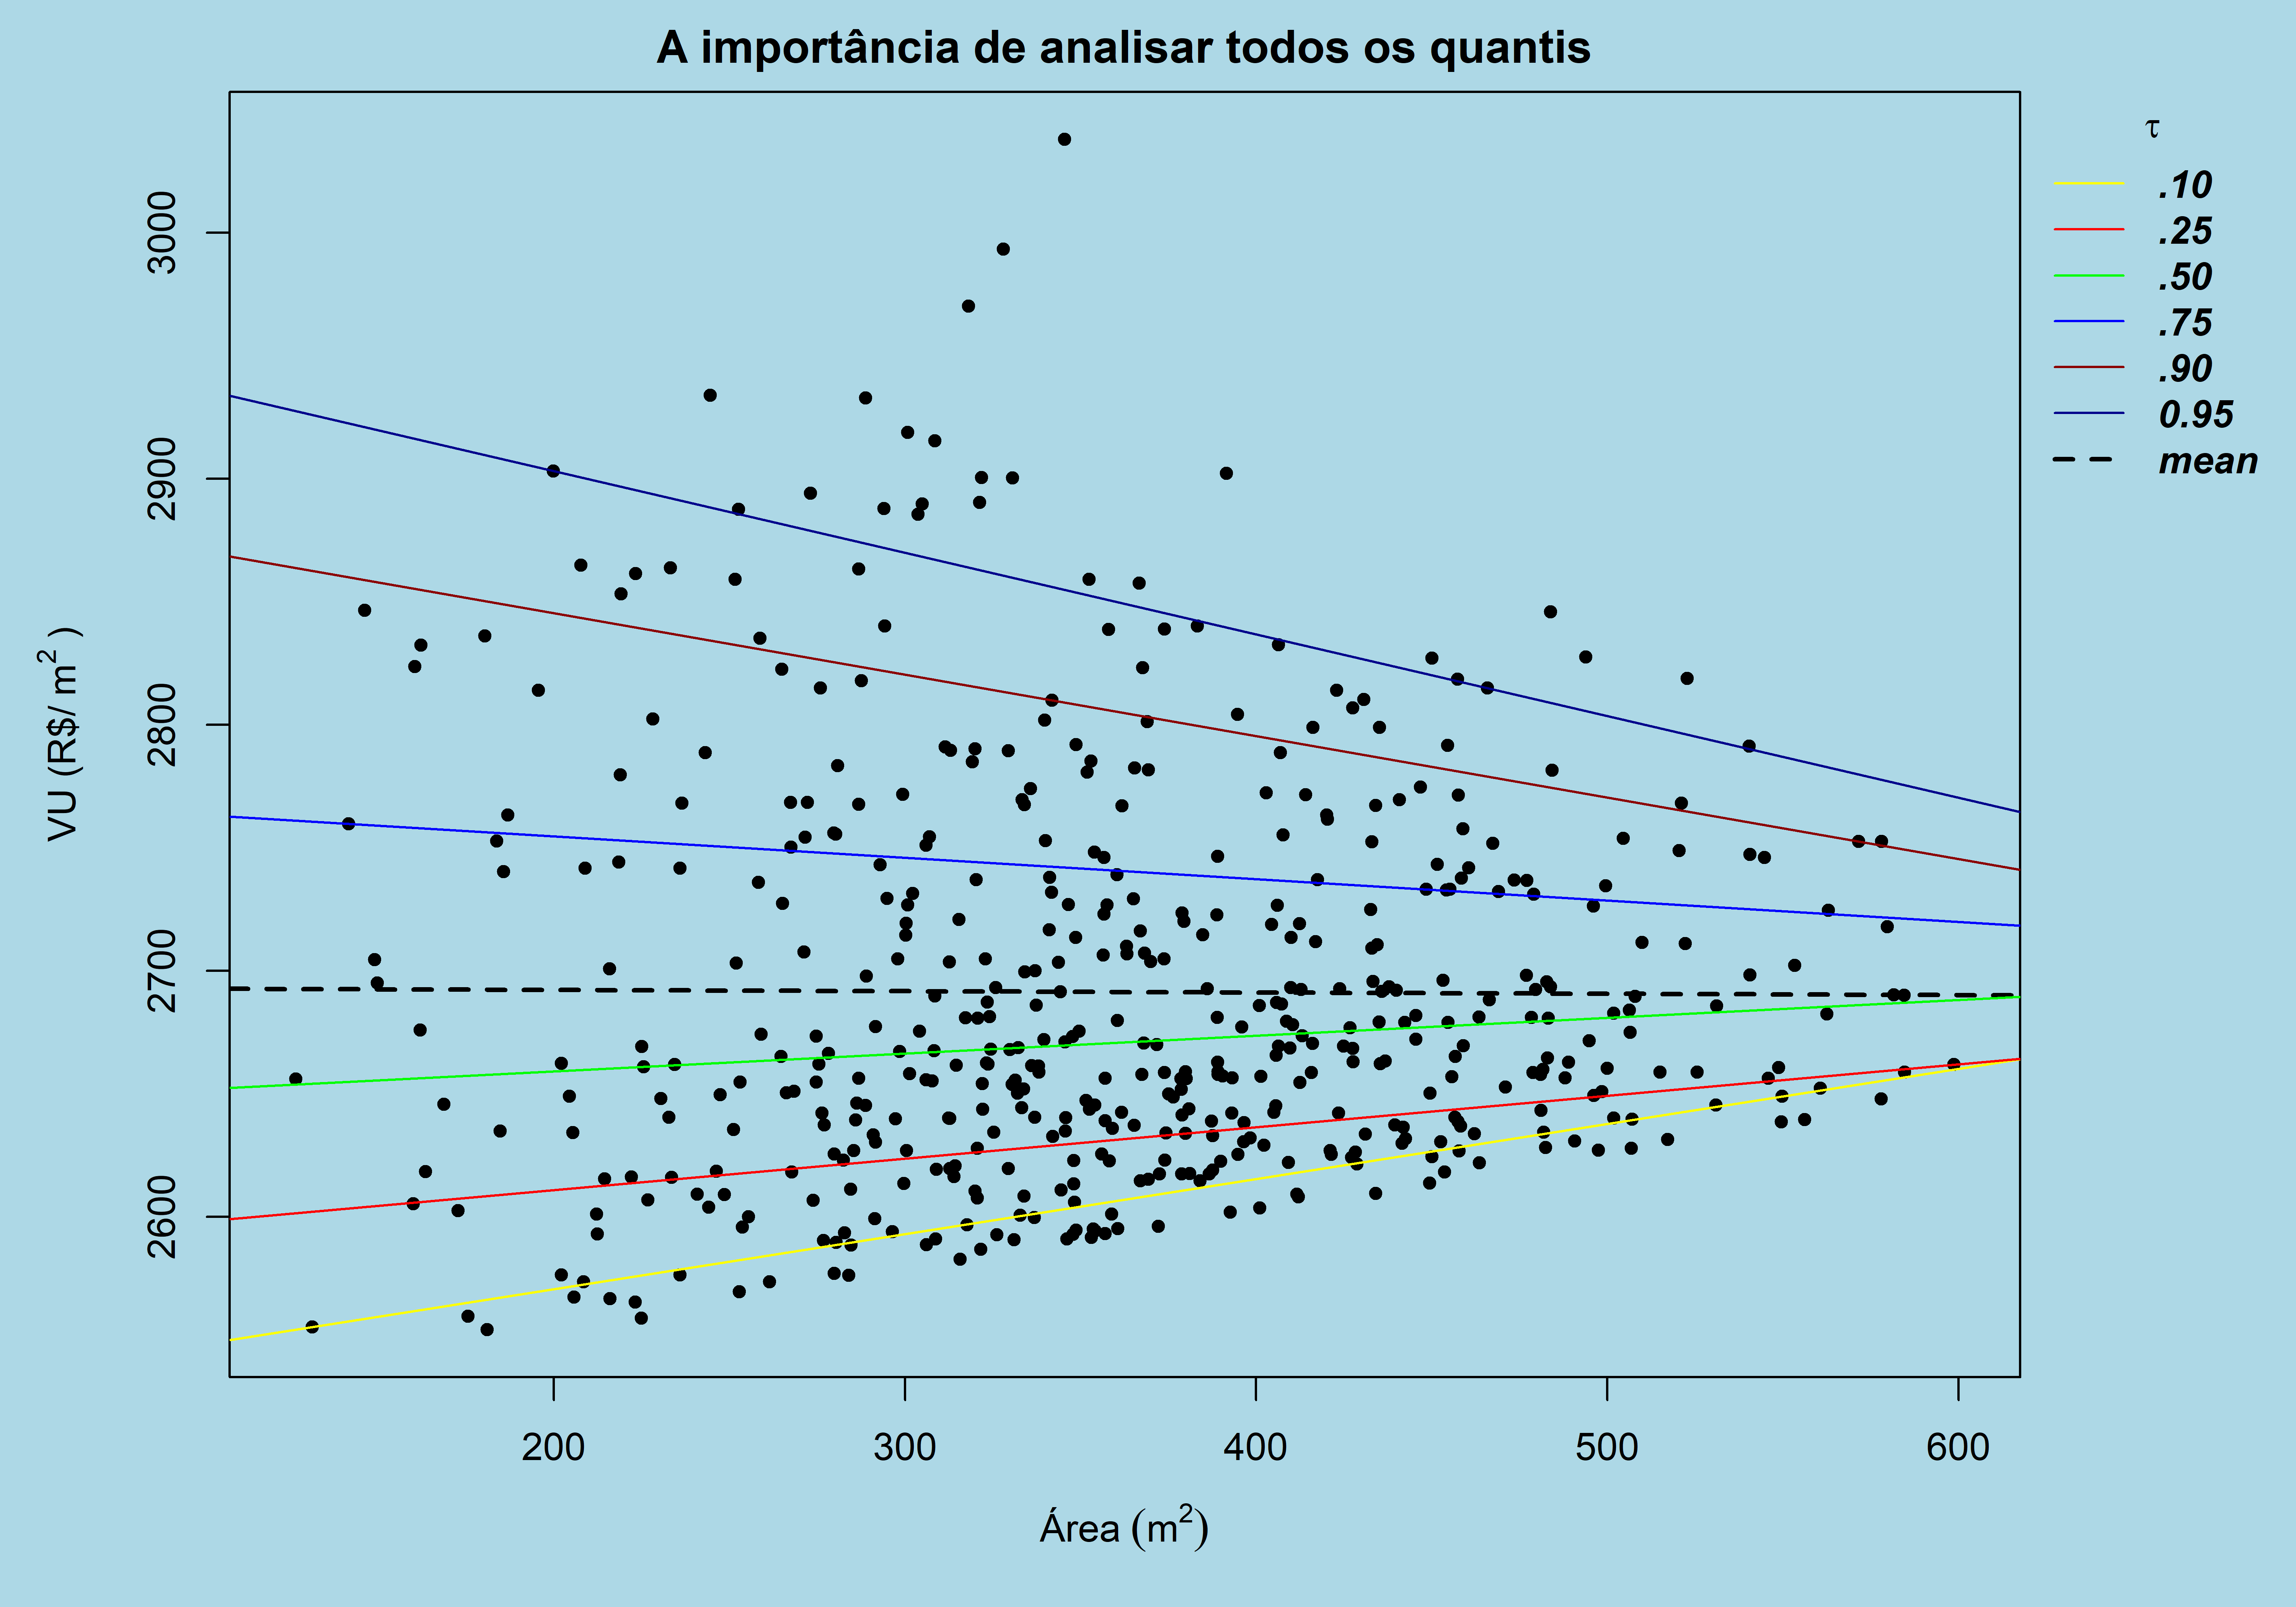
\includegraphics[width=0.5\linewidth]{images/qr-1} 

}

\caption{Regressão Quantílica.}\label{fig:qr}
\end{figure}

\end{frame}

\begin{frame}{Estimação vs.~previsão de valores}
\protect\hypertarget{estimauxe7uxe3o-vs.-previsuxe3o-de-valores-1}{}

\begin{itemize}[<+->]
\tightlist
\item
  A NBR 14.653-02\autocite{NBR1465302} parece ter também este
  entendimento:

  \begin{itemize}[<+->]
  \tightlist
  \item
    \textbf{8.2.1.5.4} O campo de arbítrio não se confunde com o
    intervalo de confiança de 80 \% calculado para definir o grau de
    precisão da estimativa.
  \end{itemize}
\item
  No Anexo A, no entanto, a NBR 14.653-02 \autocite{NBR1465302} parece
  misturar as coisas:

  \begin{itemize}[<+->]
  \item
    \textbf{A.10.1.2} Quando for adotado o valor arbitrado, o intervalo
    de valores admissíveis deve estar limitado simultaneamente (ver
    Figura A.2):\\
  \item
    \begin{enumerate}[<+->]
    [a)]
    \tightlist
    \item
      ao intervalo em torno do valor arbitrado com amplitude igual à do
      \emph{intervalo de predição \textbf{ou ao intervalo de confiança}}
      de 80\% para a estimativa de tendência central;
    \end{enumerate}
  \item
    \begin{enumerate}[<+->]
    [a)]
    \setcounter{enumi}{1}
    \tightlist
    \item
      ao campo de arbítrio em torno da estimativa de tendência central.
    \end{enumerate}
  \end{itemize}
\end{itemize}

\end{frame}

\hypertarget{por-que-arbitrar-um-valor-diferente-da-muxe9dia-condicional}{%
\section{Por que arbitrar um valor diferente da média
condicional?}\label{por-que-arbitrar-um-valor-diferente-da-muxe9dia-condicional}}

\begin{frame}{Campo de Arbítrio}
\protect\hypertarget{campo-de-arbuxedtrio}{}

\begin{itemize}[<+->]
\tightlist
\item
  \textbf{campo de arbítrio}\\
  intervalo de variação no entorno do estimador pontual adotado na
  avaliação, dentro do qual pode-se arbitrar o valor do bem,
  \textbf{desde que justificado 
  pela existência de características próprias não contempladas no modelo}.
  \autocite[3, grifo nosso]{NBR1465301}
\end{itemize}

\begin{itemize}[<+->]
\tightlist
\item
  \textbf{8.2.1.5.2} O campo de arbítrio pode ser utilizado
  \textbf{quando variáveis 
  relevantes para a avaliação do imóvel não tiverem sido contempladas no modelo},
  por escassez de dados de mercado, por inexistência de fatores de
  homogeneização aplicáveis ou porque essas variáveis não se
  apresentaram estatisticamente significantes em modelos de regressão,
  desde que a amplitude de até mais ou menos 15 \% seja suficiente para
  absorver as influências não consideradas e que os ajustes sejam
  justificados.\\
  \autocite[17, grifo nosso]{NBR1465302}
\end{itemize}

\begin{itemize}[<+->]
\tightlist
\item
  \emph{\textbf{Características próprias não contempladas no modelo}}
  \emph{vs.}
  \emph{\textbf{variáveis relevantes não contempladas no modelo.}}
\end{itemize}

\end{frame}

\begin{frame}{Problema da omissão de variável relevante}
\protect\hypertarget{problema-da-omissuxe3o-de-variuxe1vel-relevante}{}

\begin{itemize}[<+->]
\tightlist
\item
  A NBR 14.653-2 não apresenta uma definição rigorosa de \emph{variável 
  relevante}.
\item
  Seleção de variáveis é um tema complexo para o qual os estatísticos
  ainda não tem solução fechada.
\item
  Mas é consenso que, para evitar \emph{overfitting}, nem todas as
  variáveis podem ser incluídas no modelo final

  \begin{itemize}[<+->]
  \tightlist
  \item
    \(p < \sqrt{n}\) (John Tukey \emph{apud} \textcite{matloff2017})
  \end{itemize}
\item
  Mesmos variáveis com significância estatística podem ter que ser
  retiradas do modelo
\end{itemize}

\end{frame}

\begin{frame}{Além da omissão de variáveis relevantes}
\protect\hypertarget{aluxe9m-da-omissuxe3o-de-variuxe1veis-relevantes}{}

\begin{block}{Viés e Variância}

\begin{figure}

{\centering 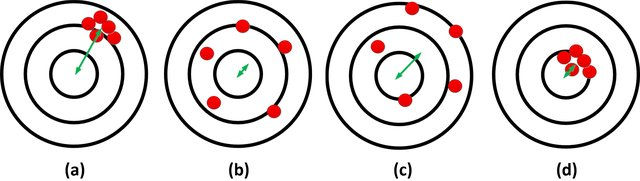
\includegraphics[width=0.7\linewidth]{../../images/The-dart-example} 

}

\caption{Viés e Variância. Fonte: \textcite{ghojogh2019theory}.}\label{fig:unnamed-chunk-2}
\end{figure}

\end{block}

\end{frame}

\begin{frame}{Tradeoff}
\protect\hypertarget{tradeoff}{}

\begin{figure}

{\centering 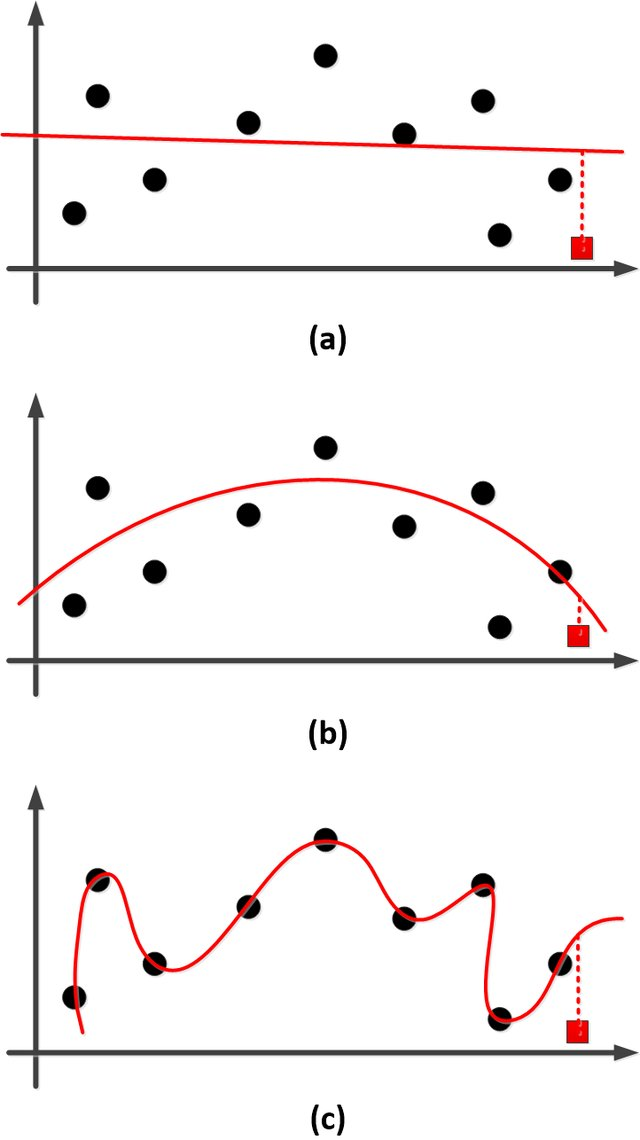
\includegraphics[width=0.25\linewidth]{../../images/An-example-for-a-underfitting-b-good-fit-and-c-overfitting-The-black-circles-and_W640} 

}

\caption{Overfitting. Fonte: \textcite{ghojogh2019theory}.}\label{fig:unnamed-chunk-3}
\end{figure}

\end{frame}

\begin{frame}{Capacidade do Modelo}
\protect\hypertarget{capacidade-do-modelo}{}

\begin{itemize}[<+->]
\tightlist
\item
  Não se pode incluir todas as variáveis
\end{itemize}

\begin{figure}

{\centering 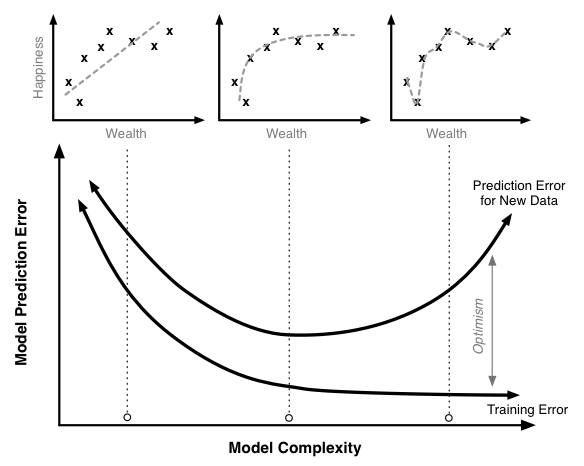
\includegraphics[width=0.4\linewidth]{../../images/model_complexity} 

}

\caption{Capacidade do modelo. Fonte: autor desconhecido.}\label{fig:unnamed-chunk-4}
\end{figure}

\begin{itemize}[<+->]
\tightlist
\item
  Moral da estória:
  \emph{If I had more time, I would have written a shorter
  letter} -- Blaise Pascal \emph{apud} \textcite{matloff2017}.
\end{itemize}

\end{frame}

\begin{frame}{Seleção de Variáveis}
\protect\hypertarget{seleuxe7uxe3o-de-variuxe1veis}{}

\end{frame}

\begin{frame}{Seleção de Variáveis}
\protect\hypertarget{seleuxe7uxe3o-de-variuxe1veis-1}{}

\begin{center}\includegraphics[width=0.7\linewidth]{../../images/modelo} \end{center}

\end{frame}

\begin{frame}{Seleção de Variáveis}
\protect\hypertarget{seleuxe7uxe3o-de-variuxe1veis-2}{}

\begin{figure}

{\centering 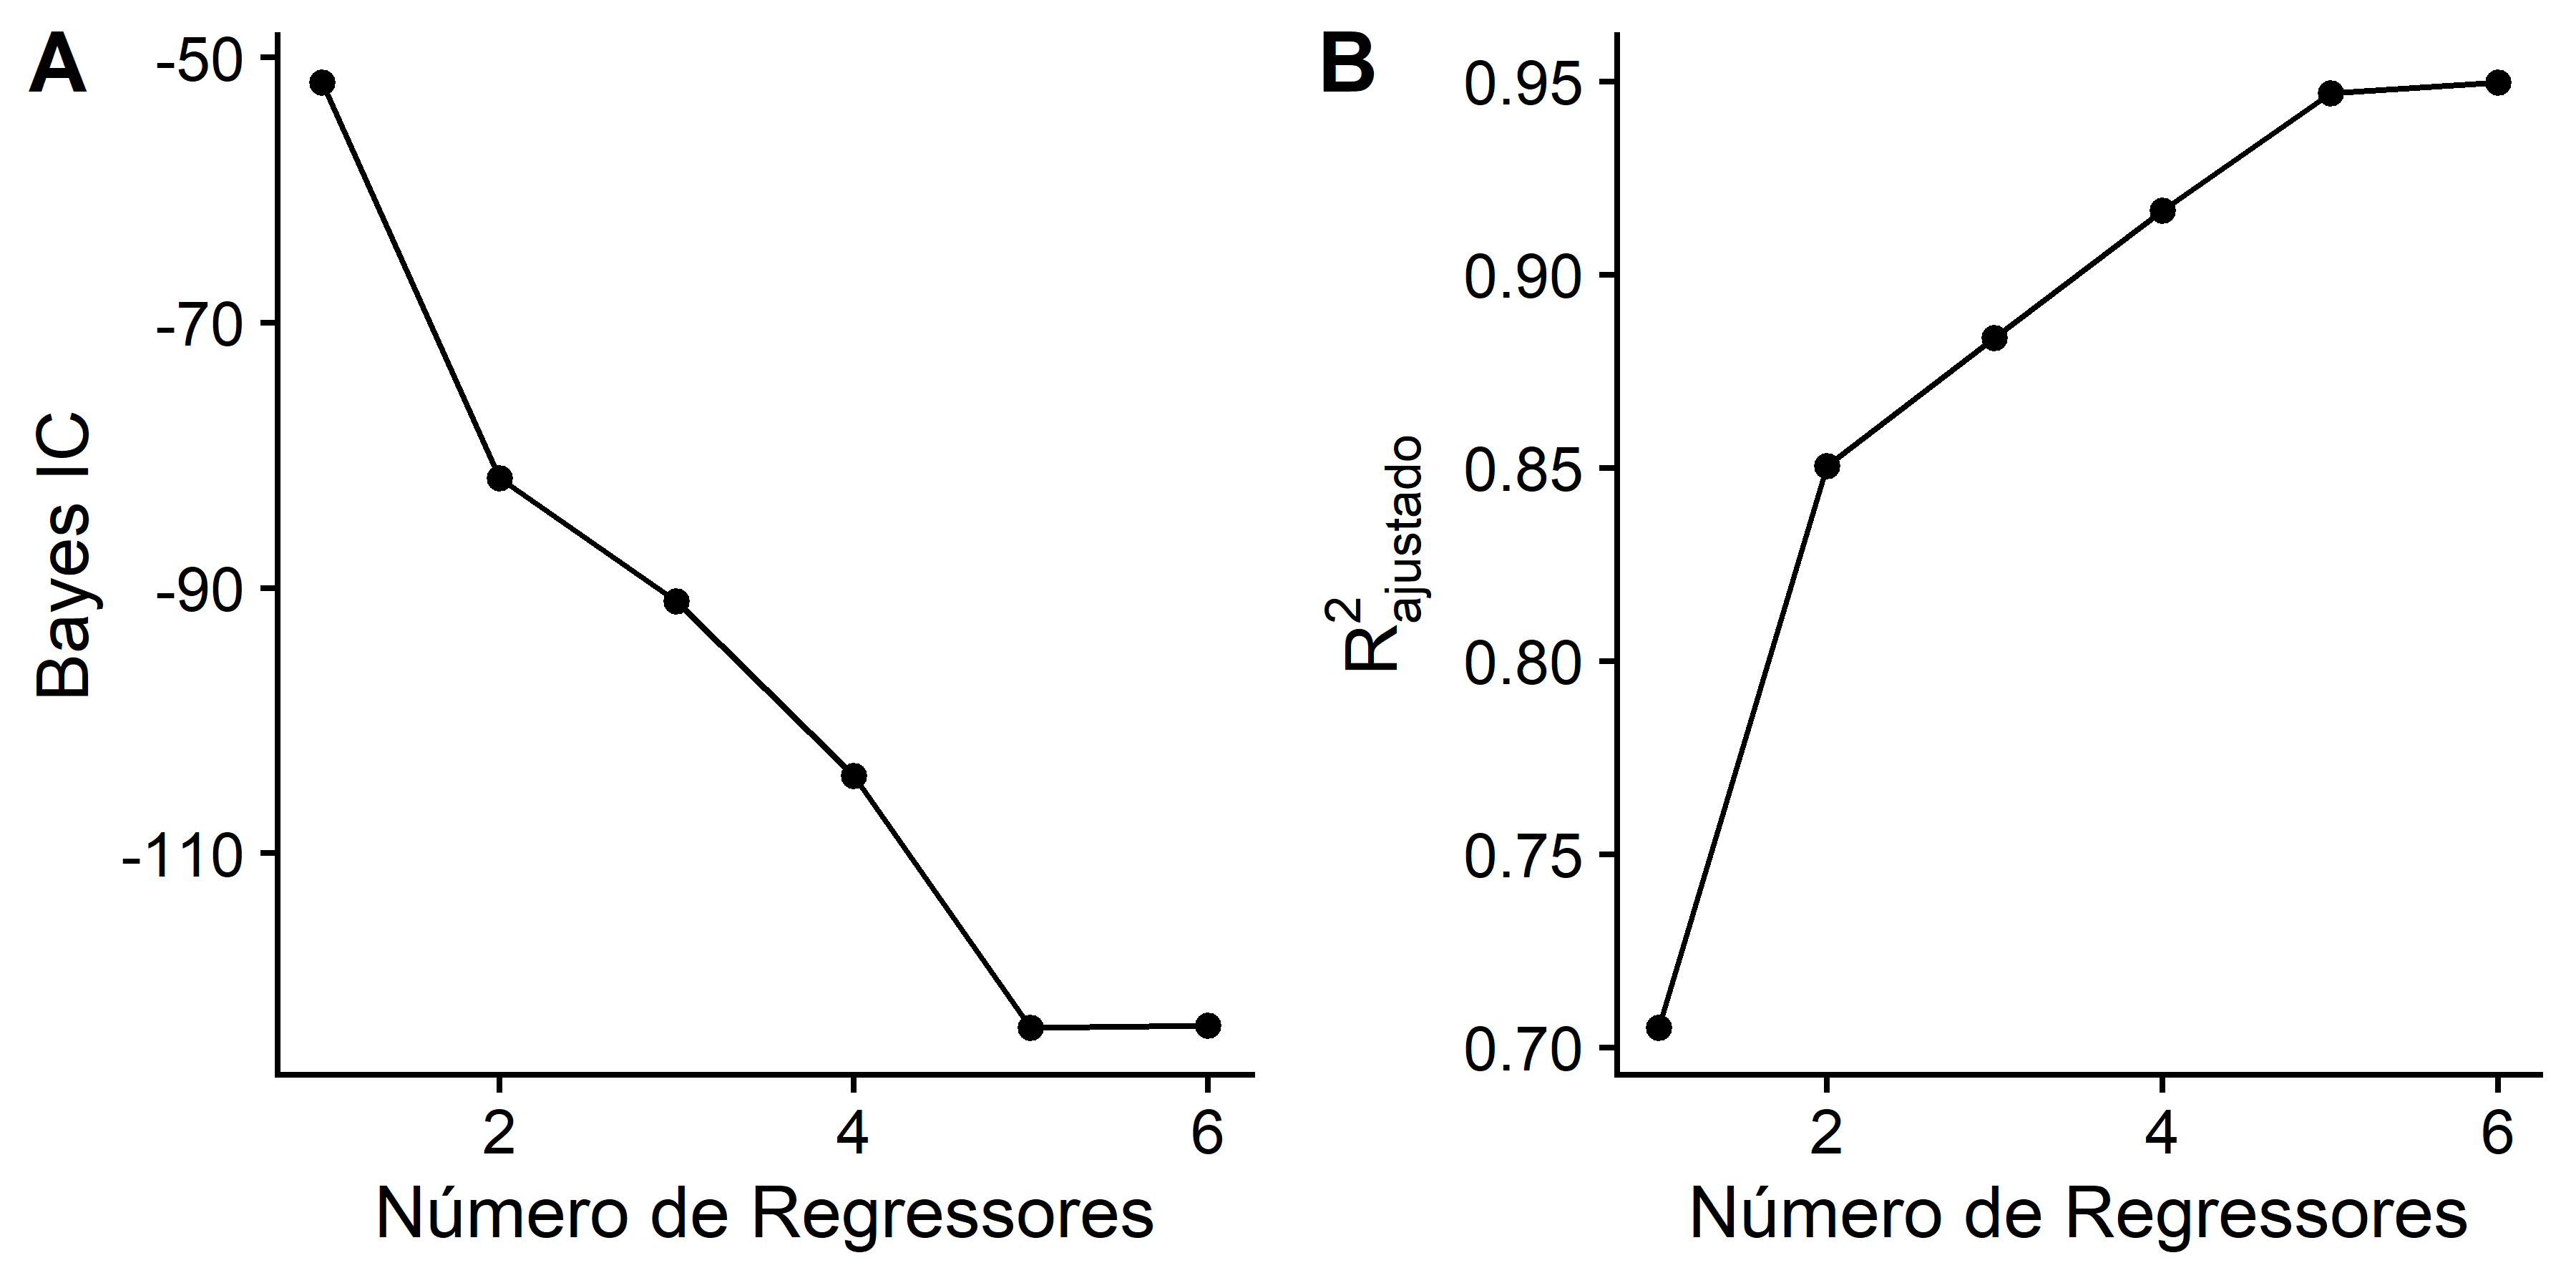
\includegraphics[width=0.8\linewidth]{images/regsub2-1} 

}

\caption{Seleção de Variáveis baseada em critérios de qualidade.}\label{fig:regsub2}
\end{figure}

\begin{itemize}[<+->]
\tightlist
\item
  Variável possui significância estatística, porém seu efeito é muito
  pequeno.
\item
  A tendência é que, com maior número de dados, mais e mais variáveis
  como esta sejam obtidas.
\end{itemize}

\end{frame}

\begin{frame}{Seleção de Variáveis}
\protect\hypertarget{seleuxe7uxe3o-de-variuxe1veis-3}{}

\begin{figure}

{\centering 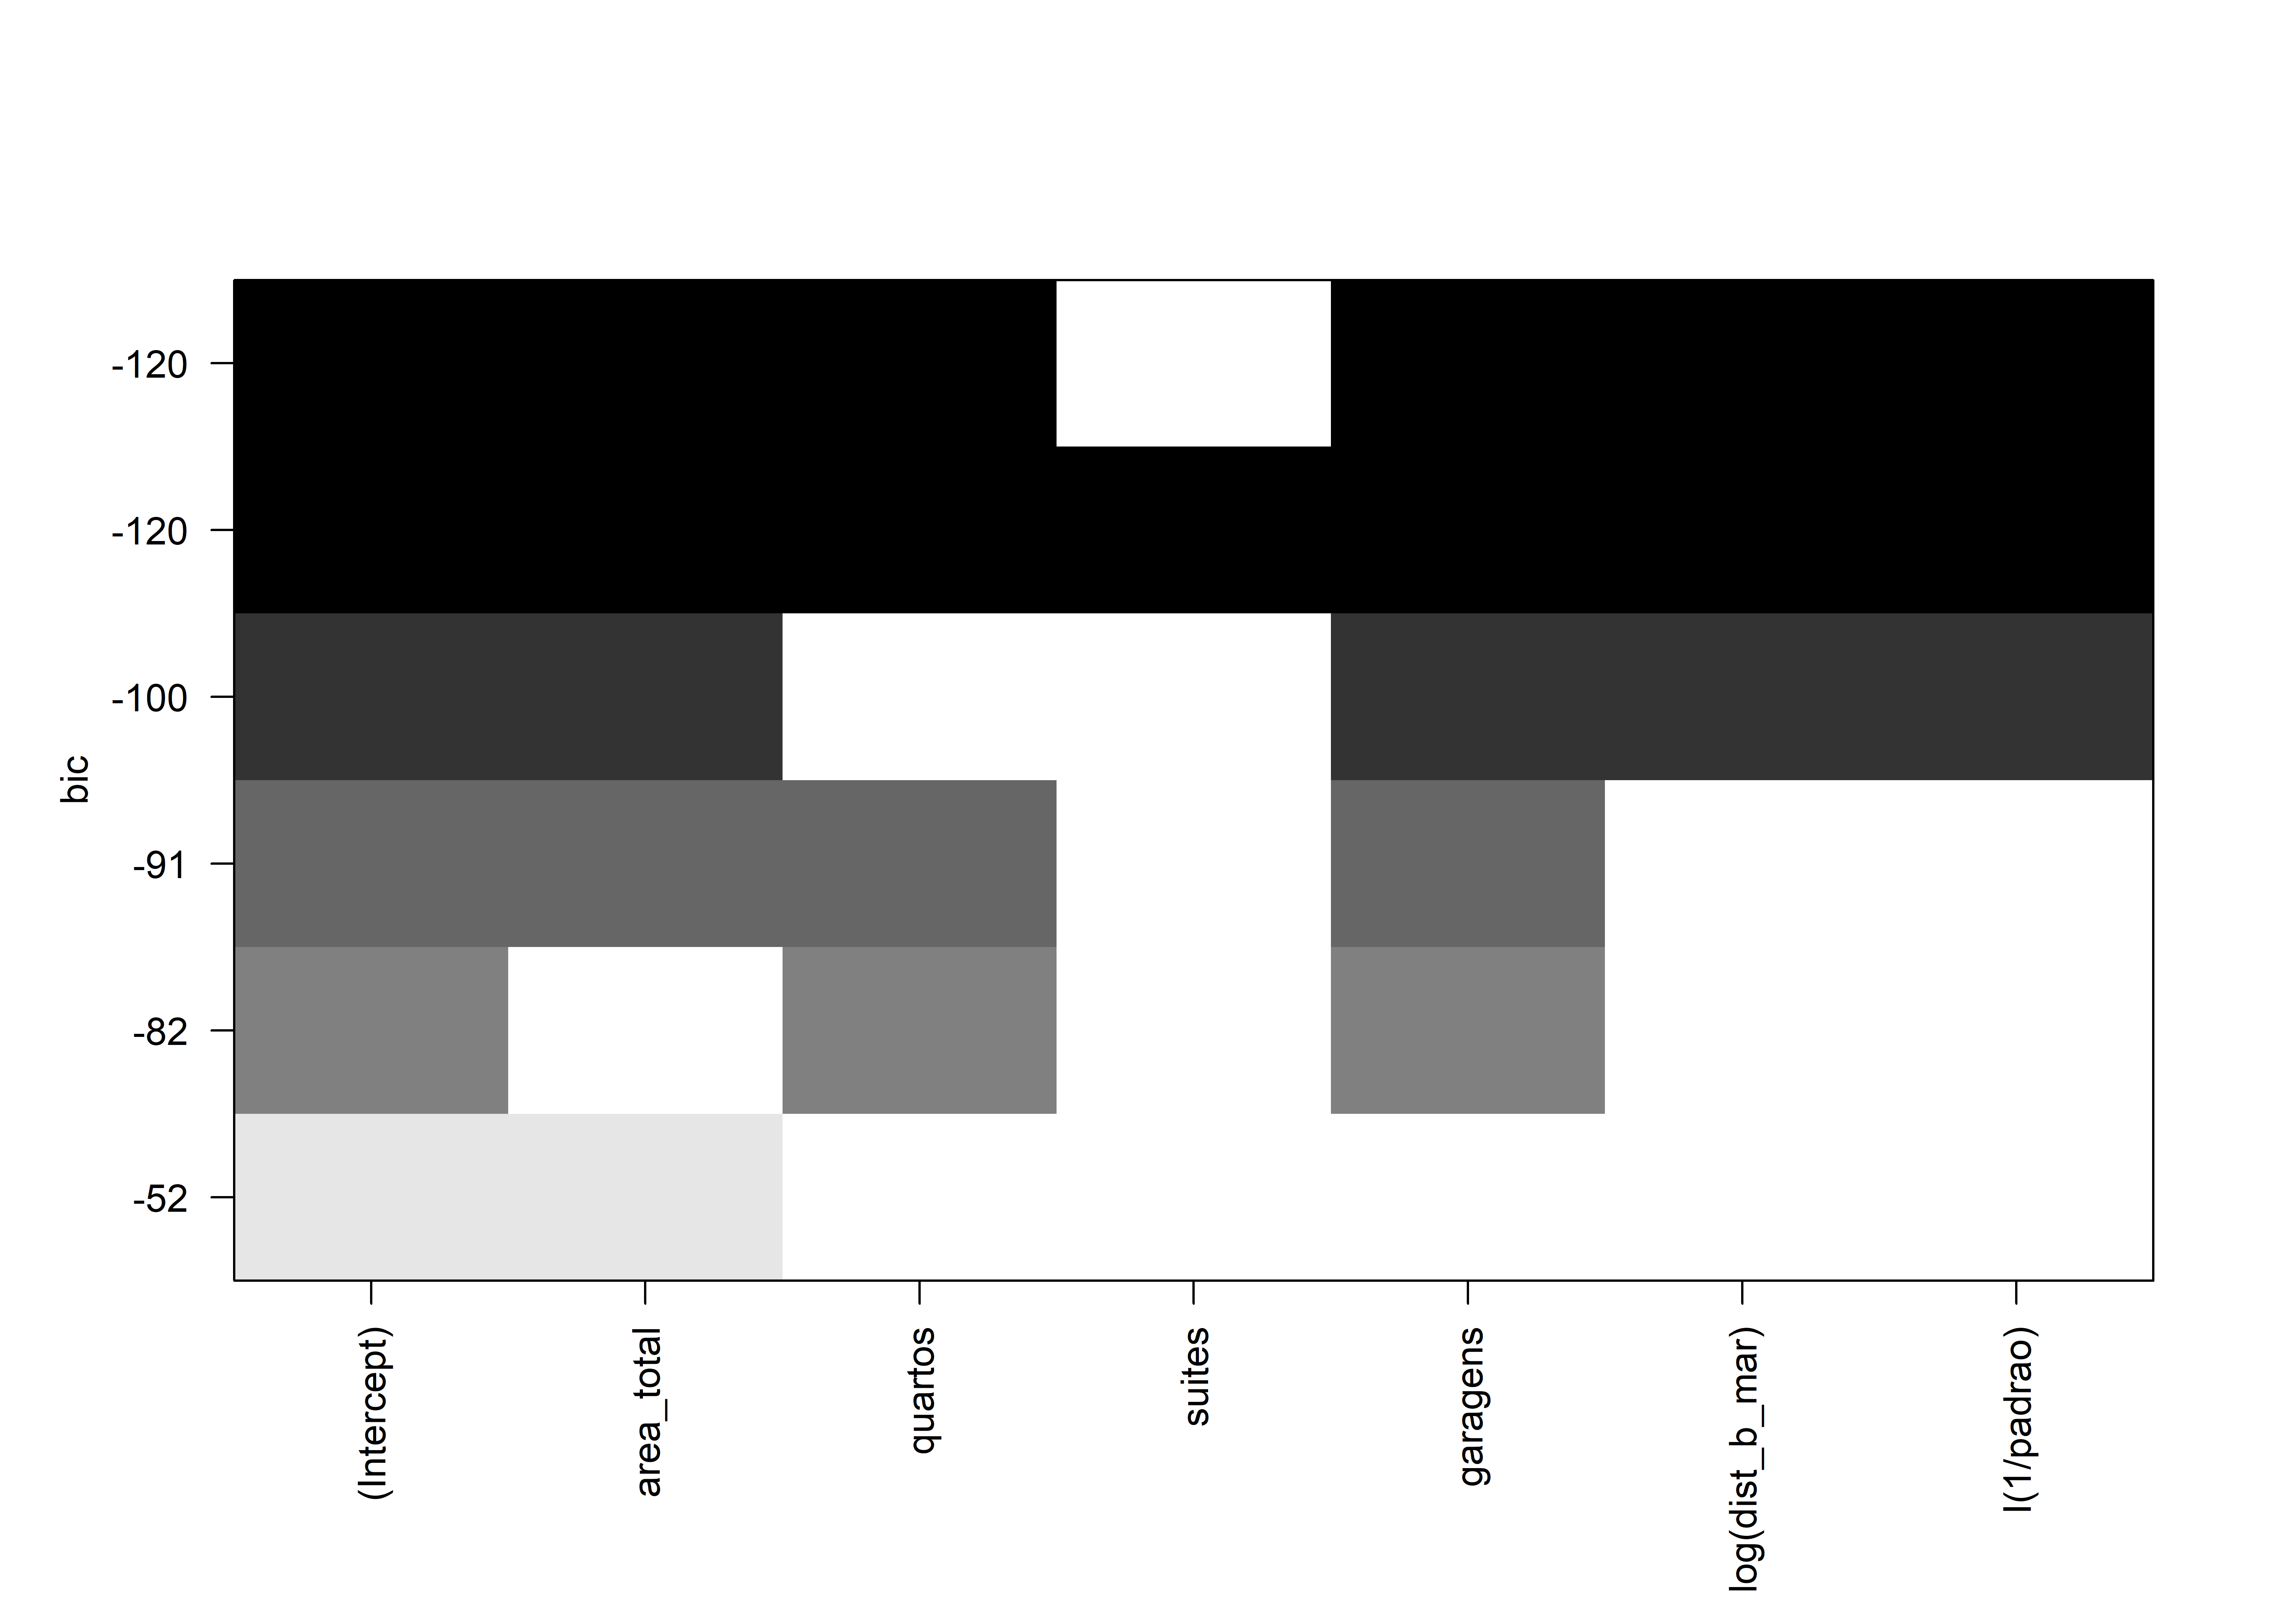
\includegraphics[width=0.7\linewidth]{images/regsub-1} 

}

\caption{Variáveis escolhidas por método exaustivo.}\label{fig:regsub}
\end{figure}

\end{frame}

\begin{frame}{Seleção de Variáveis}
\protect\hypertarget{seleuxe7uxe3o-de-variuxe1veis-4}{}

\begin{itemize}[<+->]
\tightlist
\item
  Modelo com variável suítes, IC: 961.660,64, 924.768,13, 1.000.024,94;
  Amplitude: 7,83\%
\item
  Modelo sem variável suítes, IC: 988.870,76, 955.381,88, 1.023.533,52;
  Amplitude: 6,89\%
\item
  Modelo com variável suítes, IP: 961.660,64, 802.017,63, 1.153.080,88;
  Amplitude: 36,51\%
\item
  Modelo sem variável suítes, IP: 988.870,76, 821.719,16, 1.190.023,82;
  Amplitude: 37,24\%
\end{itemize}

\begin{itemize}[<+->]
\tightlist
\item
  \textbf{There is No Panacea!}\\
\item
  Choosing a subset of predictors on the basis of cross-validation, AIC
  and so on is not foolproof by any means. Due to the Principle of
  Frequent Occurrence of Rare Events (Section 7.6.1), some subsets may
  look very good yet actually be artifacts.\\
\item
  On a theoretical basis, it has been shown that LOOM is not statiscally
  consistent {[}128{]}. That paper does find conditions under which one
  gets consistency by leaving \(w\) out rather than 1, providing
  \(w/n \rightarrow 1\), but it is not clear what the pratical
  implications are. Empirical doubt on cross-validation was cast in
  {[}118{]}.
\item
  \autocite[348]{matloff2017}
\end{itemize}

\end{frame}

\begin{frame}{Justificativa para arbitragem de valores fora da média}
\protect\hypertarget{justificativa-para-arbitragem-de-valores-fora-da-muxe9dia}{}

\begin{itemize}[<+->]
\tightlist
\item
  Na impossibilidade de se modelar todas as variáveis, cabe ao
  profissional de Engenharia de Avaliações identificar quando um imóvel
  tem valor acima ou abaixo da média do mercado estimada pelo modelo.

  \begin{itemize}[<+->]
  \tightlist
  \item
    P. ex.: Existem diversos lotes com \(A = 360m^2\) e \(F = 12m\),
    porém nem todos são iguais

    \begin{itemize}[<+->]
    \tightlist
    \item
      Um possui melhor pedologia (\(Ped\))
    \item
      Outro possui melhor Topografia (\(Topo\))
    \item
      Outro possui melhor Posição na Quadra (\(PQ\))
    \item
      Outro tem melhor Posição Solar (\(PS\))
    \item
      Devido a estas pequenas diferenças, \(\varepsilon \ne 0\)
    \item
      Porém, um lote em específico pode ter melhor
      \(Ped, Topo, PQ \,\textbf{e}\, PS\).
    \item
      Enquanto outro pode ter pior \(Ped, Topo, PQ \,\textbf{e}\, PS\).
    \item
      O valor médio estimado pelo modelo é R\$100,00/\(m^2\)
    \item
      É justo avaliá-los com o valor médio?
    \item
      Ou seria mais justo utilizar o primeiro e o nono decil da
      distribuição de probabilidades?
    \end{itemize}
  \end{itemize}
\end{itemize}

\end{frame}

\hypertarget{estudos-de-casos}{%
\section{Estudos de casos}\label{estudos-de-casos}}

\begin{frame}{Omissão de variável relevante}
\protect\hypertarget{omissuxe3o-de-variuxe1vel-relevante}{}

\begin{figure}

{\centering 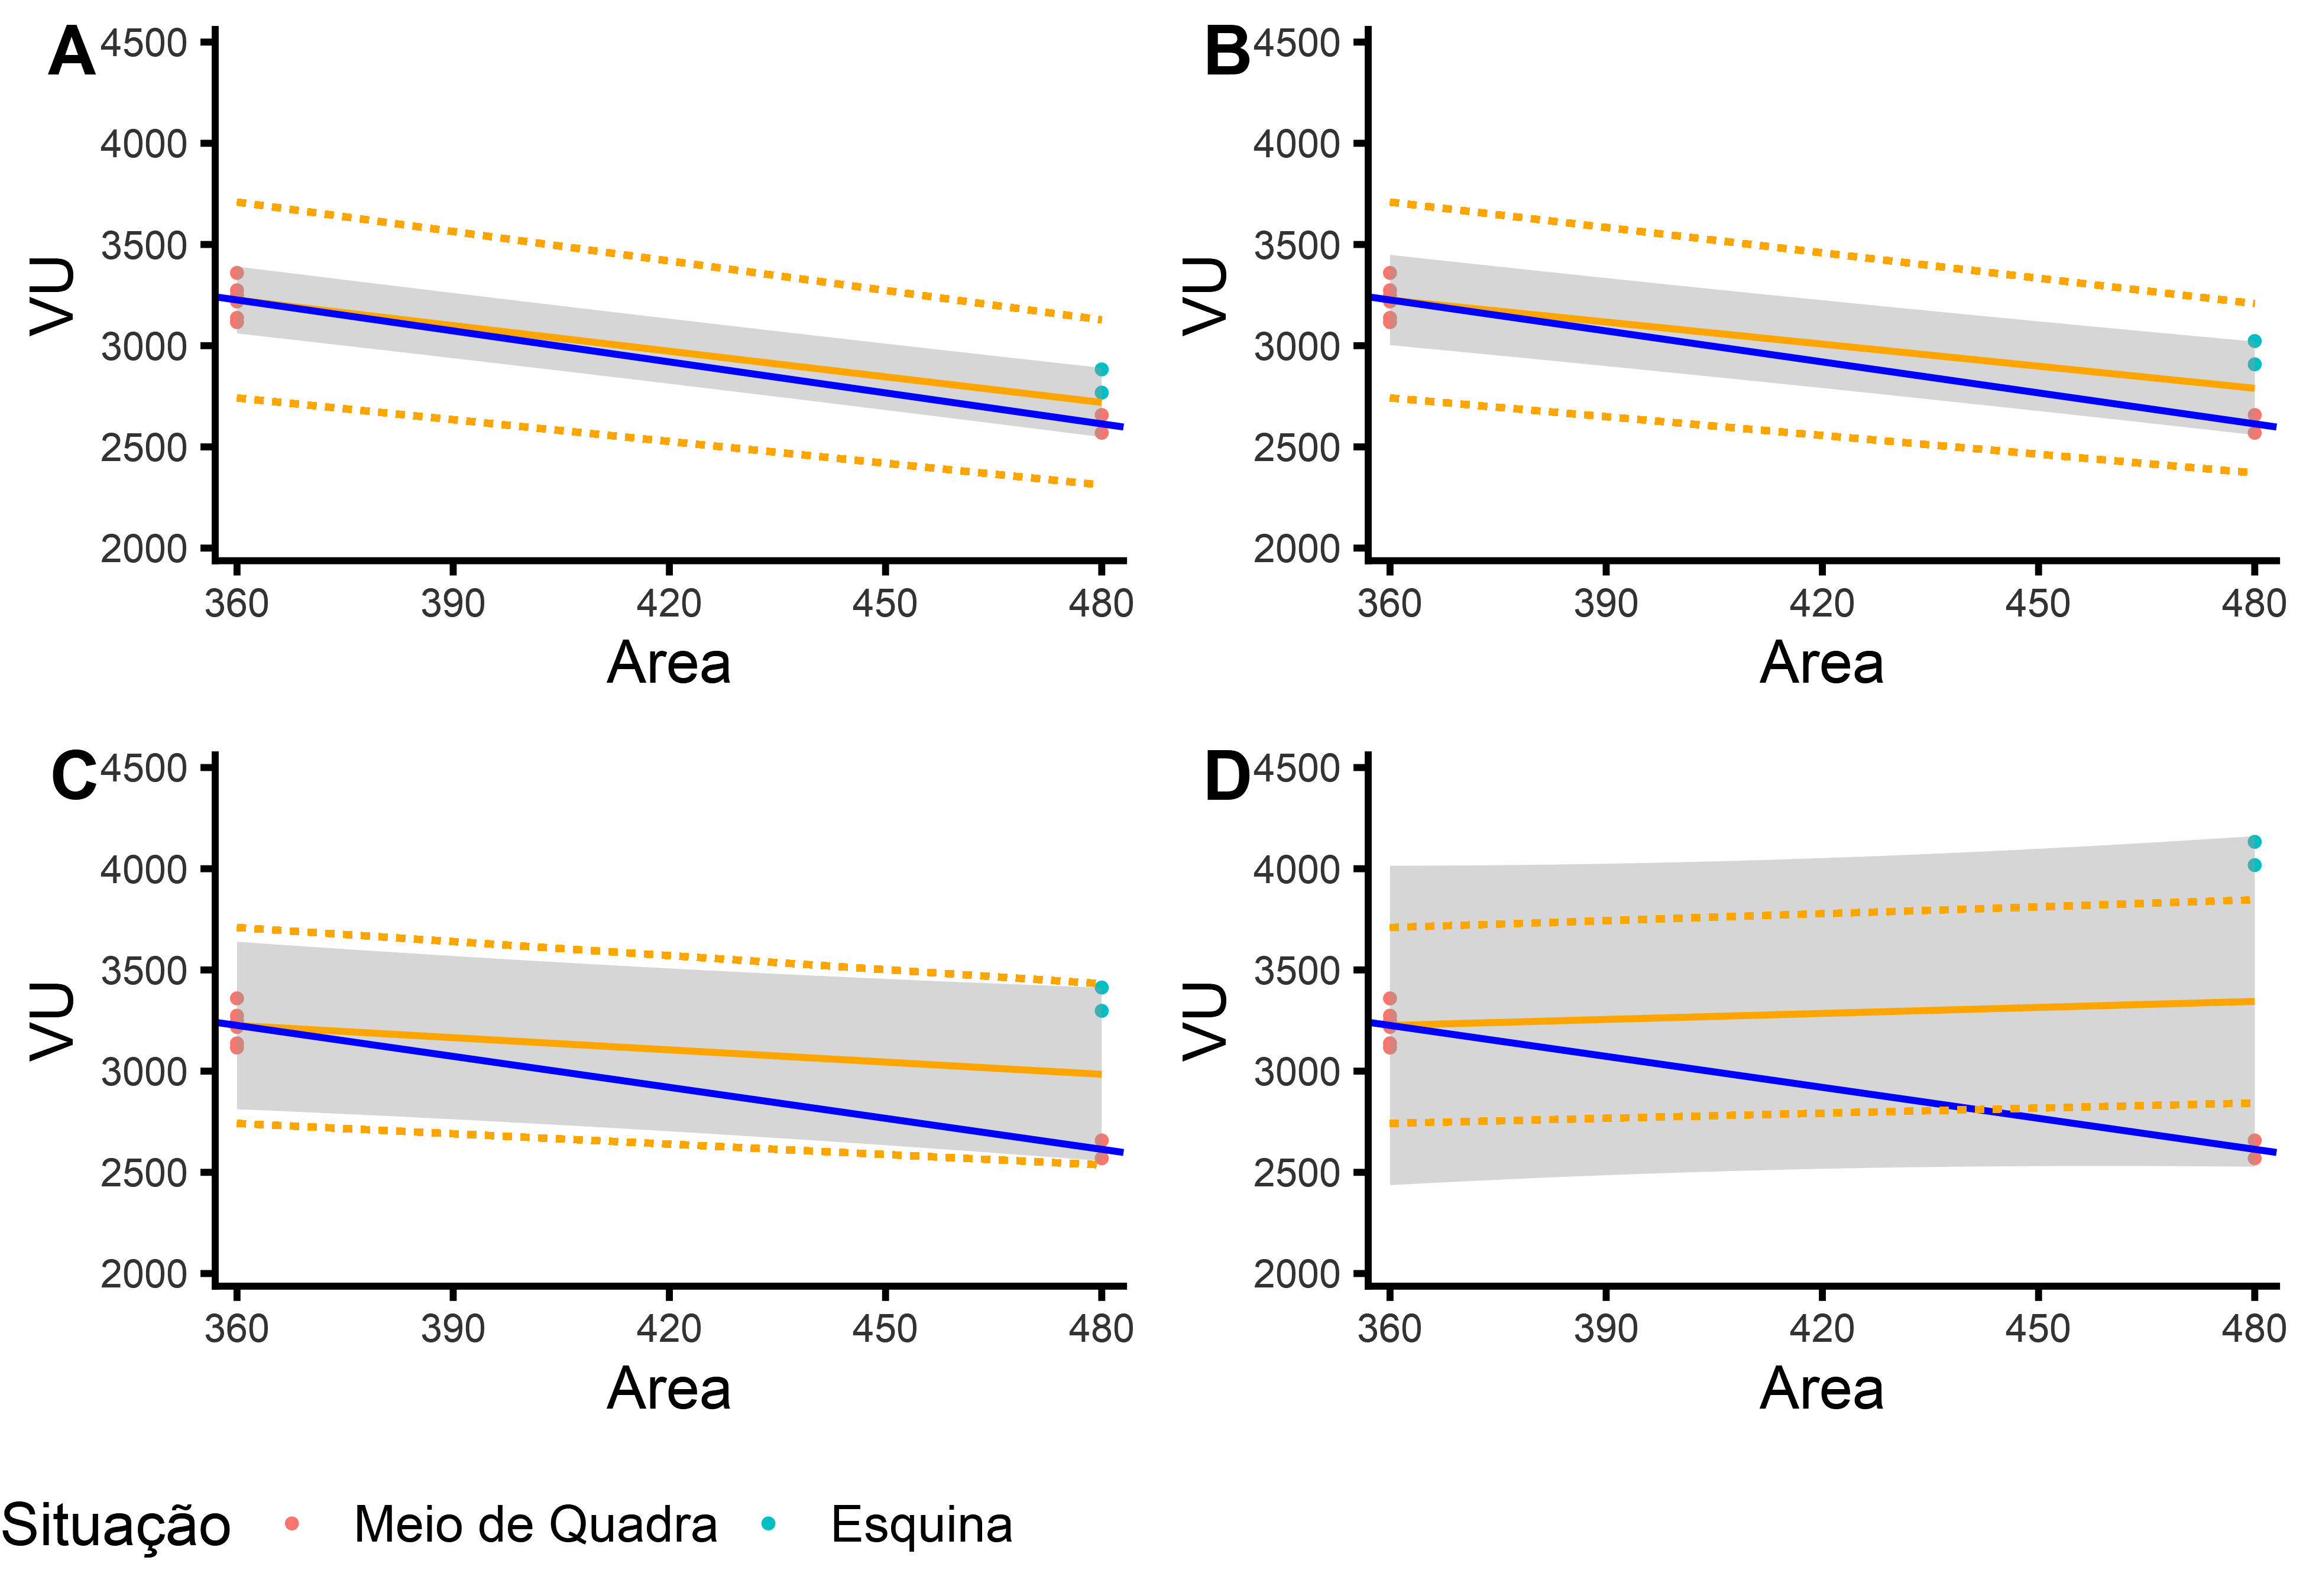
\includegraphics[width=0.7\linewidth]{../../images/modelos-1} 

}

\caption{Omissão de variável relevante: quatro exemplos ilustrativos. Fonte: os autores.}\label{fig:unnamed-chunk-8}
\end{figure}

\end{frame}

\begin{frame}{Omissão de variável relevante}
\protect\hypertarget{omissuxe3o-de-variuxe1vel-relevante-1}{}

\begin{itemize}
\tightlist
\item
  Qual o valor de um lote dado que \(A = 480 \, e\, PQ = 1\)
\end{itemize}

\begin{itemize}[<+->]
\tightlist
\item
  A NBR 14.653-2 prevê a utilização do CA
\item
  Entendemos que o CA pode ser um bom fator limitante
\item
  Mas não dá qualquer parâmetro para a previsão de valores

  \begin{itemize}[<+->]
  \tightlist
  \item
    P. Ex.: Lote em situação de esquina, sem variável situação
  \item
    Pode-se utilizar o CA. Mas em qual magnitude?
  \item
    Quanto a posição na quadra valoriza o lote em relação à situação de
    meio-de-quadra?
  \item
    Intervalos de Predição podem ser instrutivos
  \end{itemize}
\end{itemize}

\end{frame}

\begin{frame}{Micronumerosidade}
\protect\hypertarget{micronumerosidade}{}

\begin{itemize}[<+->]
\tightlist
\item
  \alert<1>{Modelo sem micronumerosidade}
\end{itemize}

\begin{figure}

{\centering 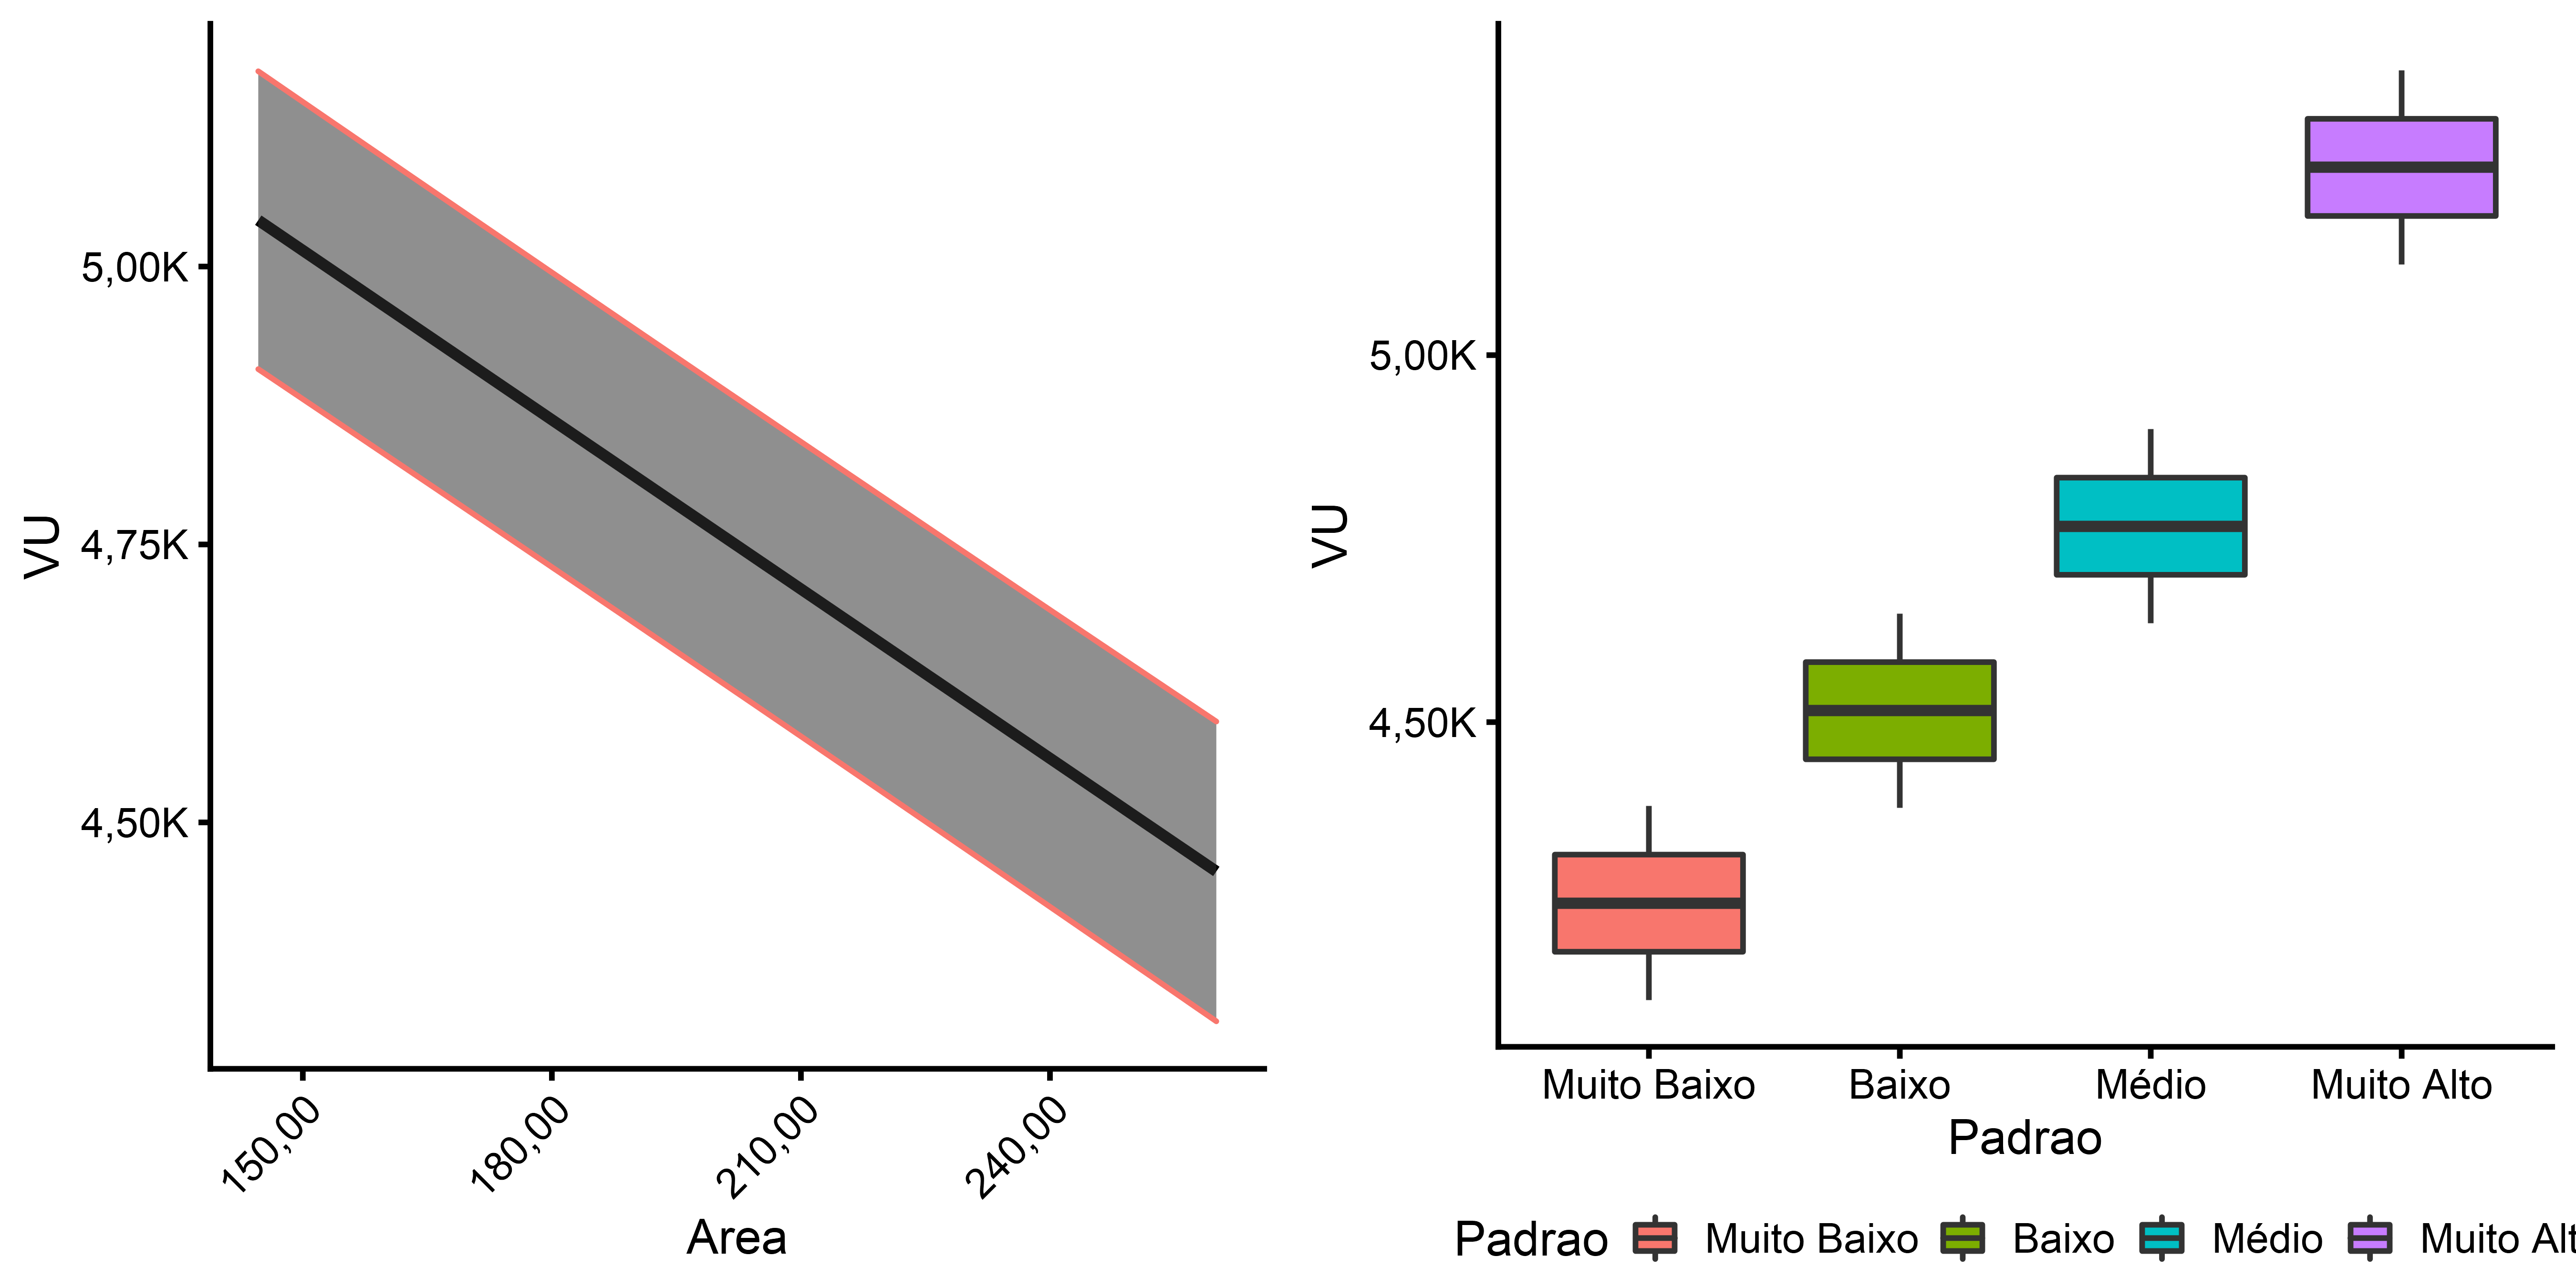
\includegraphics[width=0.7\linewidth]{../../images/modelo-1} 

}

\caption{Micronumerosidade: perda de informação no modelo. Fonte: os autores.}\label{fig:unnamed-chunk-9}
\end{figure}

\begin{itemize}[<+->]
\tightlist
\item
  \alert<2>{Quanto vale imóvel de Padrão Alto? (Com código alocado seria possível \cite[A.6]{NBR1465302})}
\end{itemize}

\end{frame}

\begin{frame}{Micronumerosidade (2)}
\protect\hypertarget{micronumerosidade-2}{}

\begin{itemize}[<+->]
\tightlist
\item
  \alert<1>{Modelo com poucos dados de padrão alto (<3)}
\end{itemize}

\begin{figure}

{\centering 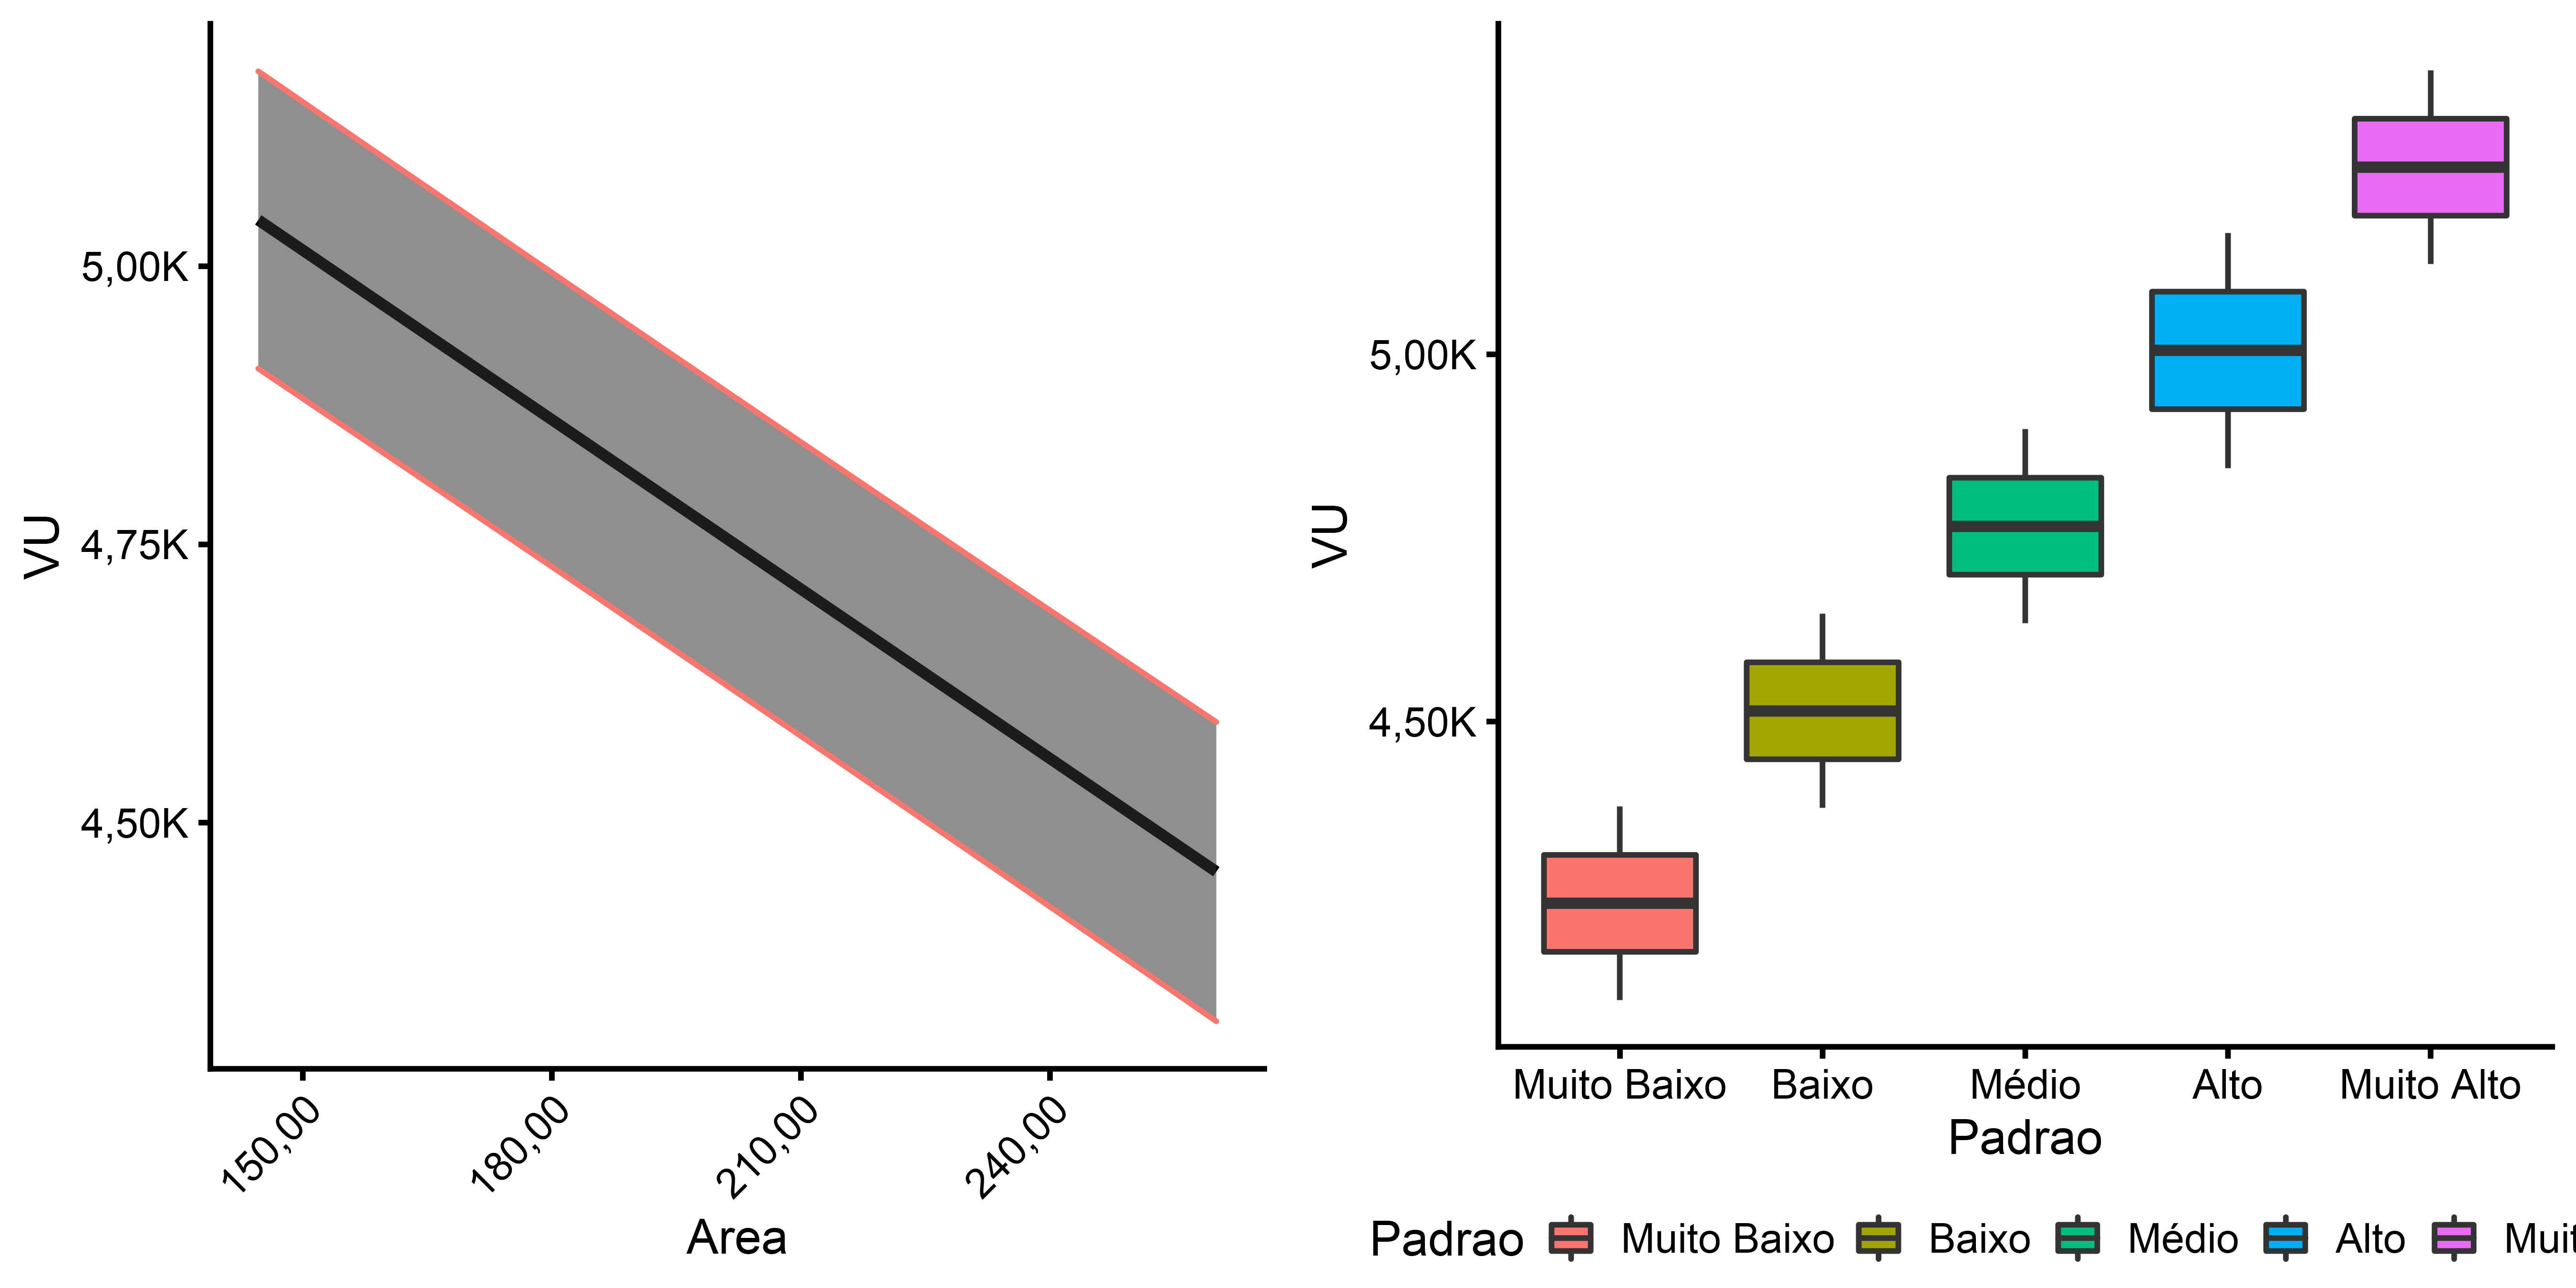
\includegraphics[width=0.7\linewidth]{../../images/modelo1-1} 

}

\caption{Pequeno número de dados: Estimação pobre. Fonte: os autores.}\label{fig:unnamed-chunk-10}
\end{figure}

\begin{itemize}[<+->]
\tightlist
\item
  \alert<2>{$Var(VU|Padrao = Alto) > Var(VU| Padrao \ne Alto)$. Se atende GP, por que não?}
\end{itemize}

\end{frame}

\begin{frame}{Avaliação Intervalar}
\protect\hypertarget{avaliauxe7uxe3o-intervalar}{}

\begin{figure}

{\centering 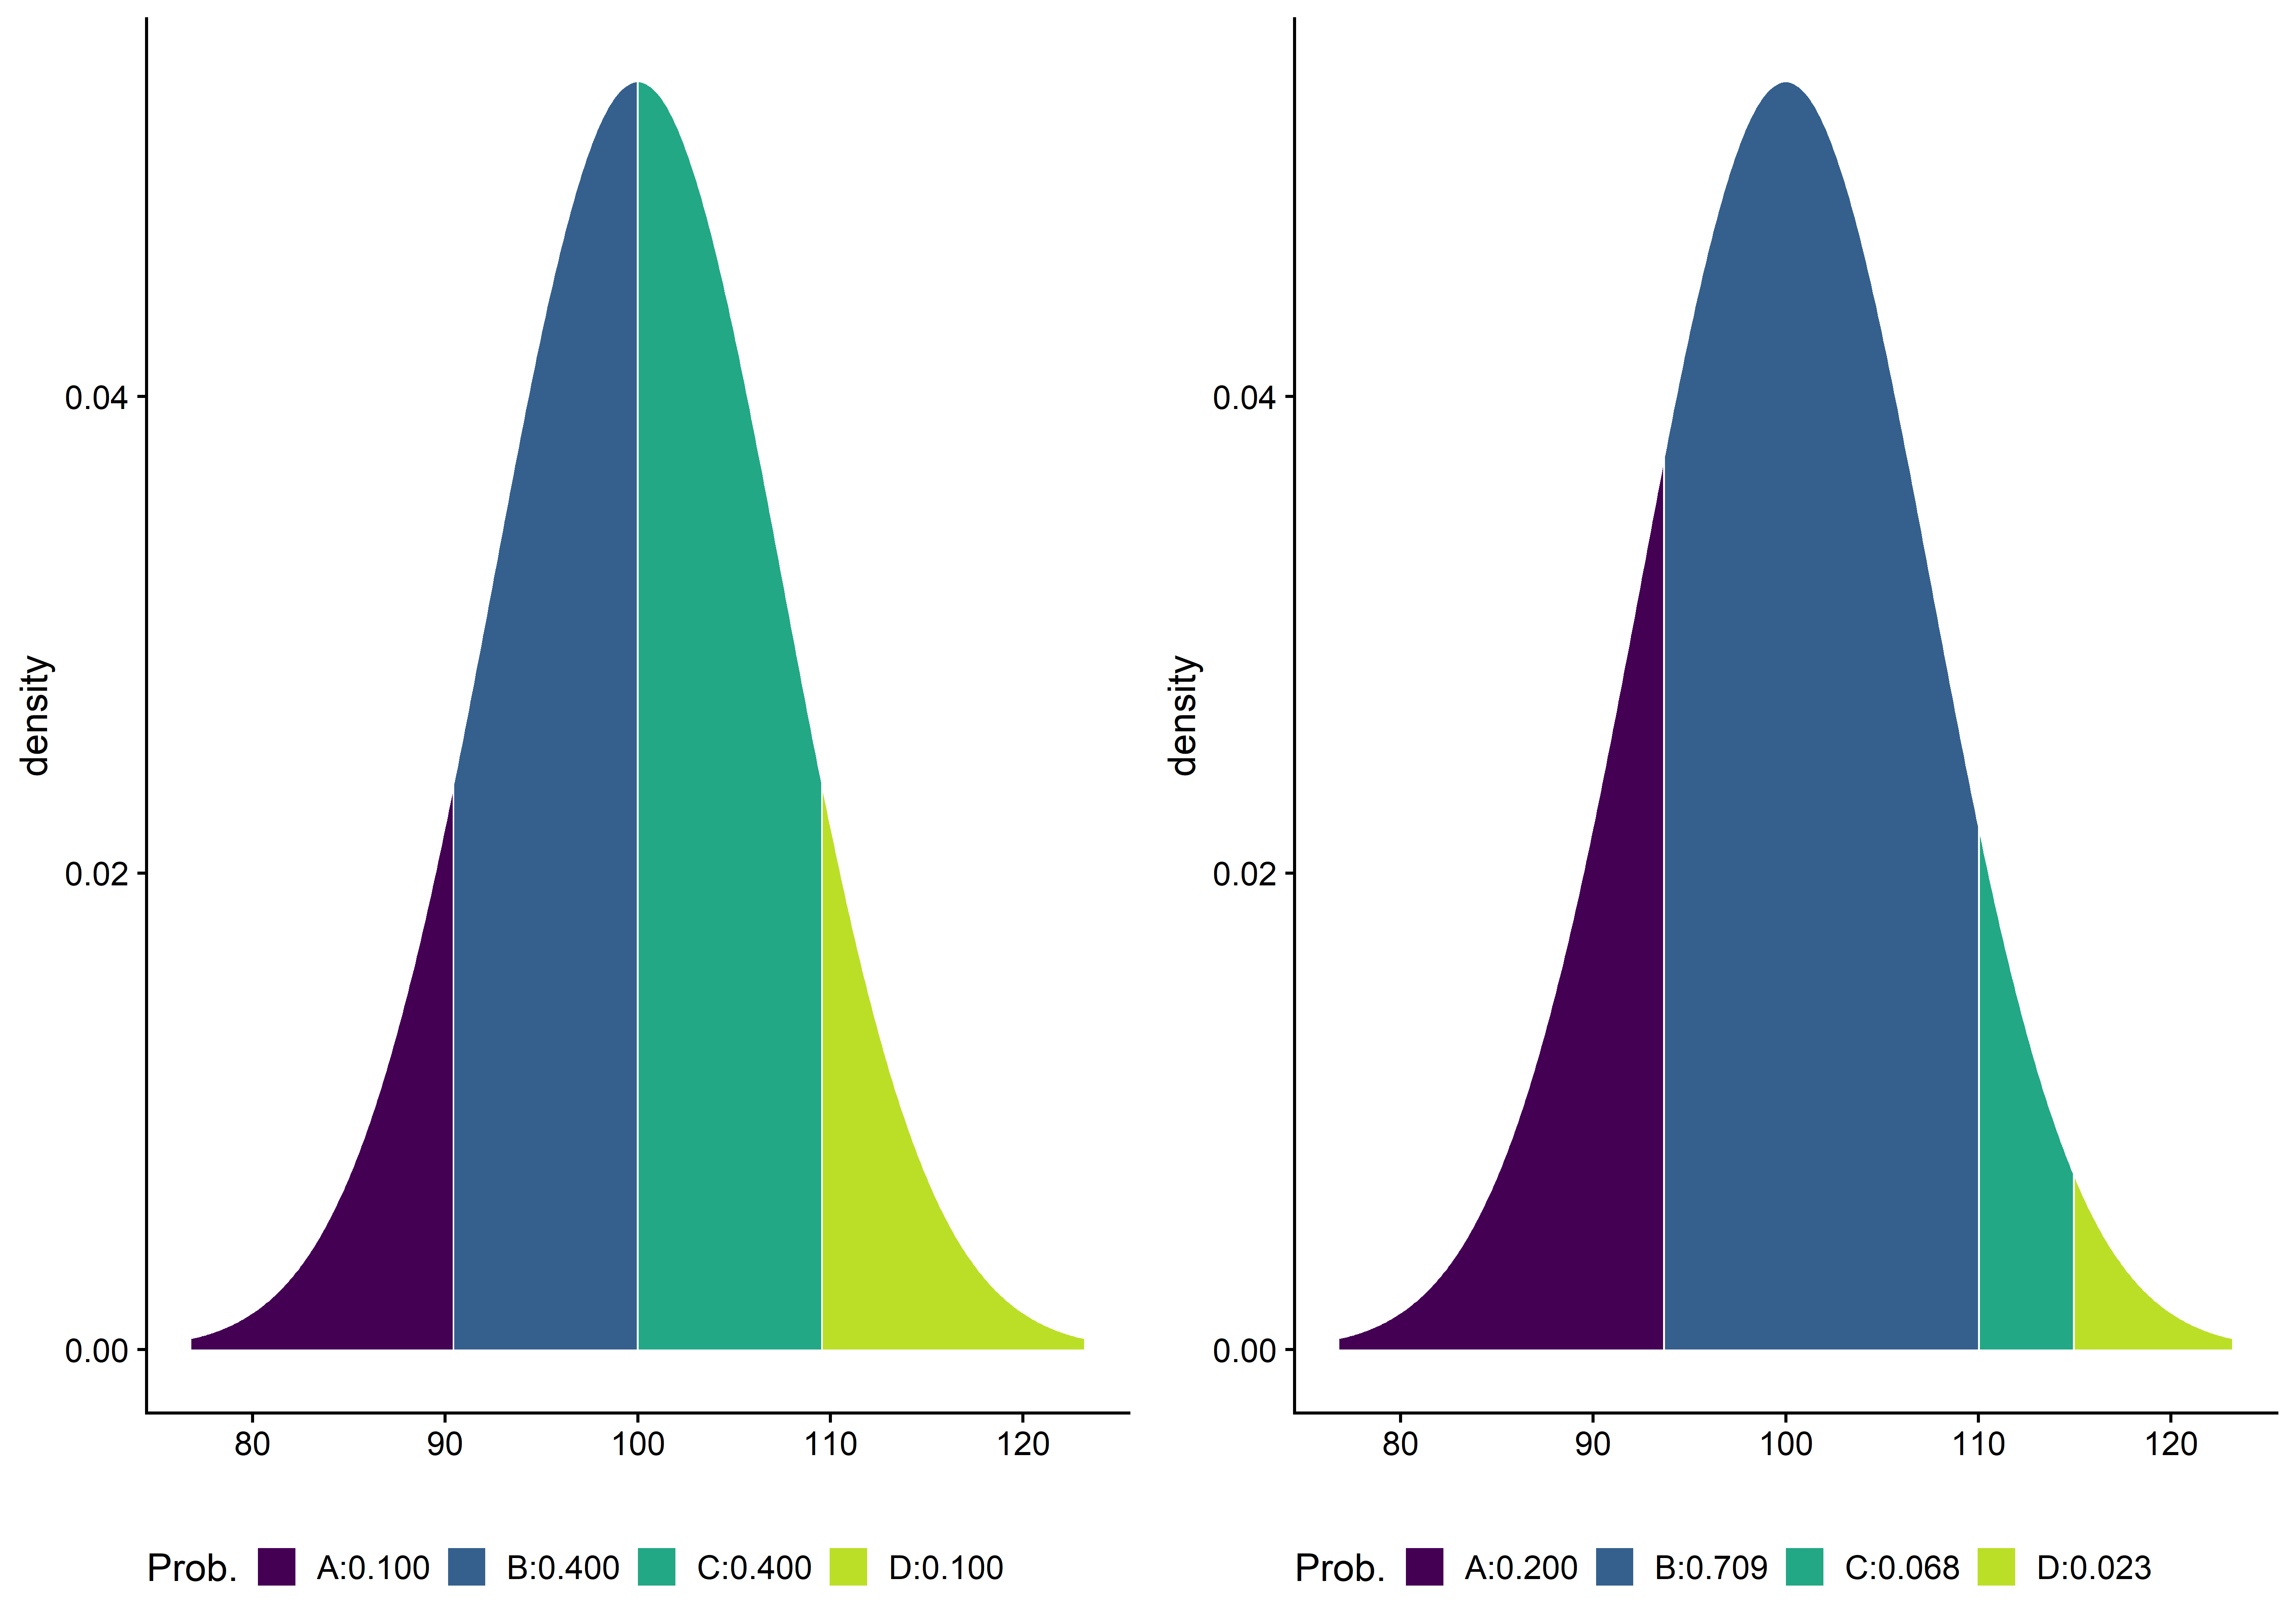
\includegraphics[width=0.5\linewidth]{images/avalInterv-1} 

}

\caption{Avaliação Intervalar. Intervalos incoerentes.}\label{fig:avalInterv}
\end{figure}

\begin{itemize}[<+->]
\tightlist
\item
  Faz sentido arbitrar um valor maior do que a média e reportar um
  intervalo admissível com valores abaixo da média?
\end{itemize}

\end{frame}

\begin{frame}{Avaliação Intervalar (2)}
\protect\hypertarget{avaliauxe7uxe3o-intervalar-2}{}

\begin{figure}

{\centering 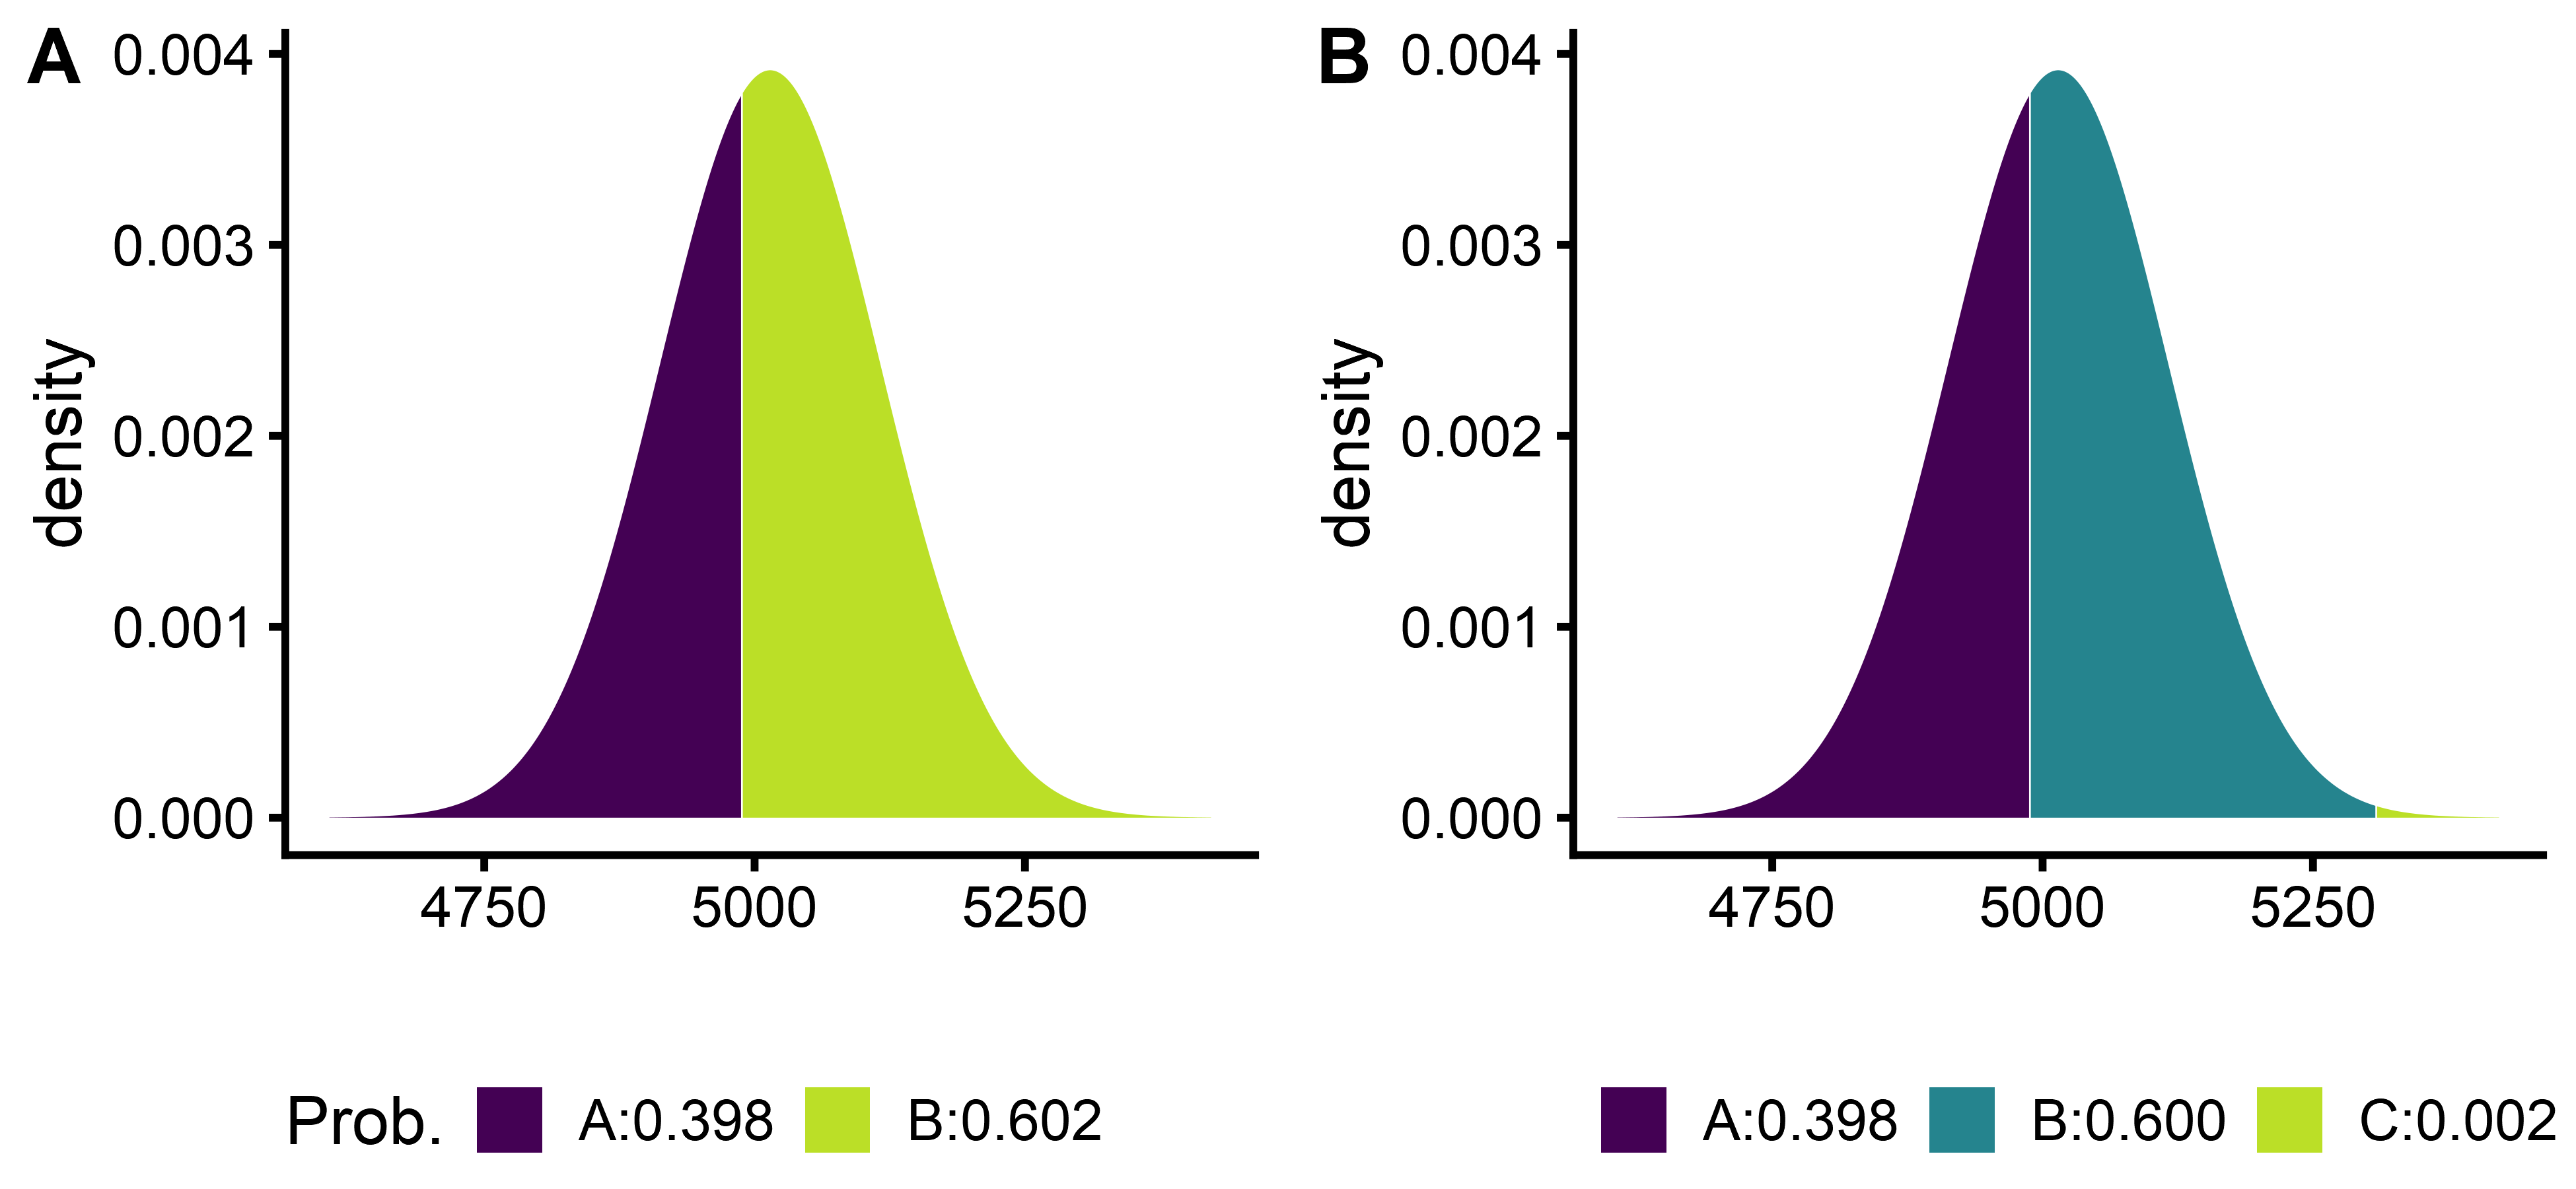
\includegraphics[width=0.7\linewidth]{../../images/dists-1} 

}

\caption{Estimação intervalar: uma abordagem probabilística. Fonte: os autores.}\label{fig:unnamed-chunk-11}
\end{figure}

\begin{itemize}[<+->]
\tightlist
\item
  Arbitragem de valor acima da média:

  \begin{itemize}[<+->]
  \tightlist
  \item
    valores admissíveis: \([IC_{inf}; CA_{sup}]\) ou
    \([IC_{inf}; IP_{sup}]\)
  \item
    valores admissíveis: \([IC_{inf}; min(CA_{sup}, IP_{sup})]\)
  \item
    valores admissíveis:
    \(Y_{arb} \pm min(Y_{arb} - IC_{inf}; min(IP_{sup}, CA_{sup}) - Y_{arb})\)
    (simétrico)
  \end{itemize}
\end{itemize}

\end{frame}

\hypertarget{conclusuxf5es}{%
\section{Conclusões}\label{conclusuxf5es}}

\begin{frame}{Conclusões}

\begin{itemize}[<+->]
\tightlist
\item
  \alert<1>{O campo de arbítrio (CA) é um artifício que possibilita ao 
  avaliador a escolha de um valor para o bem-avaliando diferente do valor (médio) 
  ajustado com o modelo de regressão linear.}
\end{itemize}

\begin{itemize}[<+->]
\tightlist
\item
  \alert<2>{A NBR 14653-2 \citeyear{NBR1465302} permite que o CA seja 
  utilizado apenas quando da omissão de variável relevante. Esta exigência não 
  consta na NBR 14653-1 \citeyear{NBR1465301}.}
\end{itemize}

\begin{itemize}[<+->]
\tightlist
\item
  \alert<3>{O cálculo do IP é um bom parâmetro para estimar o \emph{quanto} o 
  valor do bem pode/deve ser majorado ou minorado.}
\end{itemize}

\begin{itemize}[<+->]
\tightlist
\item
  \alert<4>{O IC não é um bom parâmetro para a arbitragem de valores para novos
  dados (fora da amostra).}
\end{itemize}

\begin{itemize}[<+->]
\tightlist
\item
  \alert<5>{O CA deve ser utilizado, portanto, como um fator limitante, 
  \textbf{em conjunto com o IP!}}
\end{itemize}

\begin{itemize}[<+->]
\tightlist
\item
  \alert<6>{A micronumerosidade deveria ser revista. Deixar que os dados falem!}
\end{itemize}

\end{frame}


  \begin{frame}[allowframebreaks]{Referências}
  \bibliographytrue
  \printbibliography[heading=none]
  \end{frame}


\end{document}
